\documentclass[10pt]{beamer}

\usetheme[progressbar=frametitle]{metropolis}
\usepackage{appendixnumberbeamer}

\usepackage{booktabs}
\usepackage[scale=2]{ccicons}
\usepackage[portuguese]{babel}

\usepackage{pgfplots}
\usepgfplotslibrary{dateplot}

\usepackage{xspace}
\newcommand{\themename}{\textbf{\textsc{metropolis}}\xspace}

\title{Geração Procedural de Terrenos para Jogos}
% \subtitle{A modern beamer theme}
\date{\today}
% \date{}
\author{João Carlos Becker}
% \institute{Center for modern beamer themes}
% \titlegraphic{\hfill\includegraphics[height=1.5cm]{logo.pdf}}

\begin{document}

\maketitle

% Qual o problema? porque é bom ter geração procedural terrenos
% \section{Introdução}

\begin{frame}{Contextualização}
  \begin{itemize}
        \item Criar conteúdo para jogos manualmente exige muito tempo de trabalho
        \item Conteúdo criado manualmente exige persistência do próprio conteúdo
    \end{itemize}
\end{frame}

\begin{frame}{Contextualização}
    \begin{figure}
		\centering
        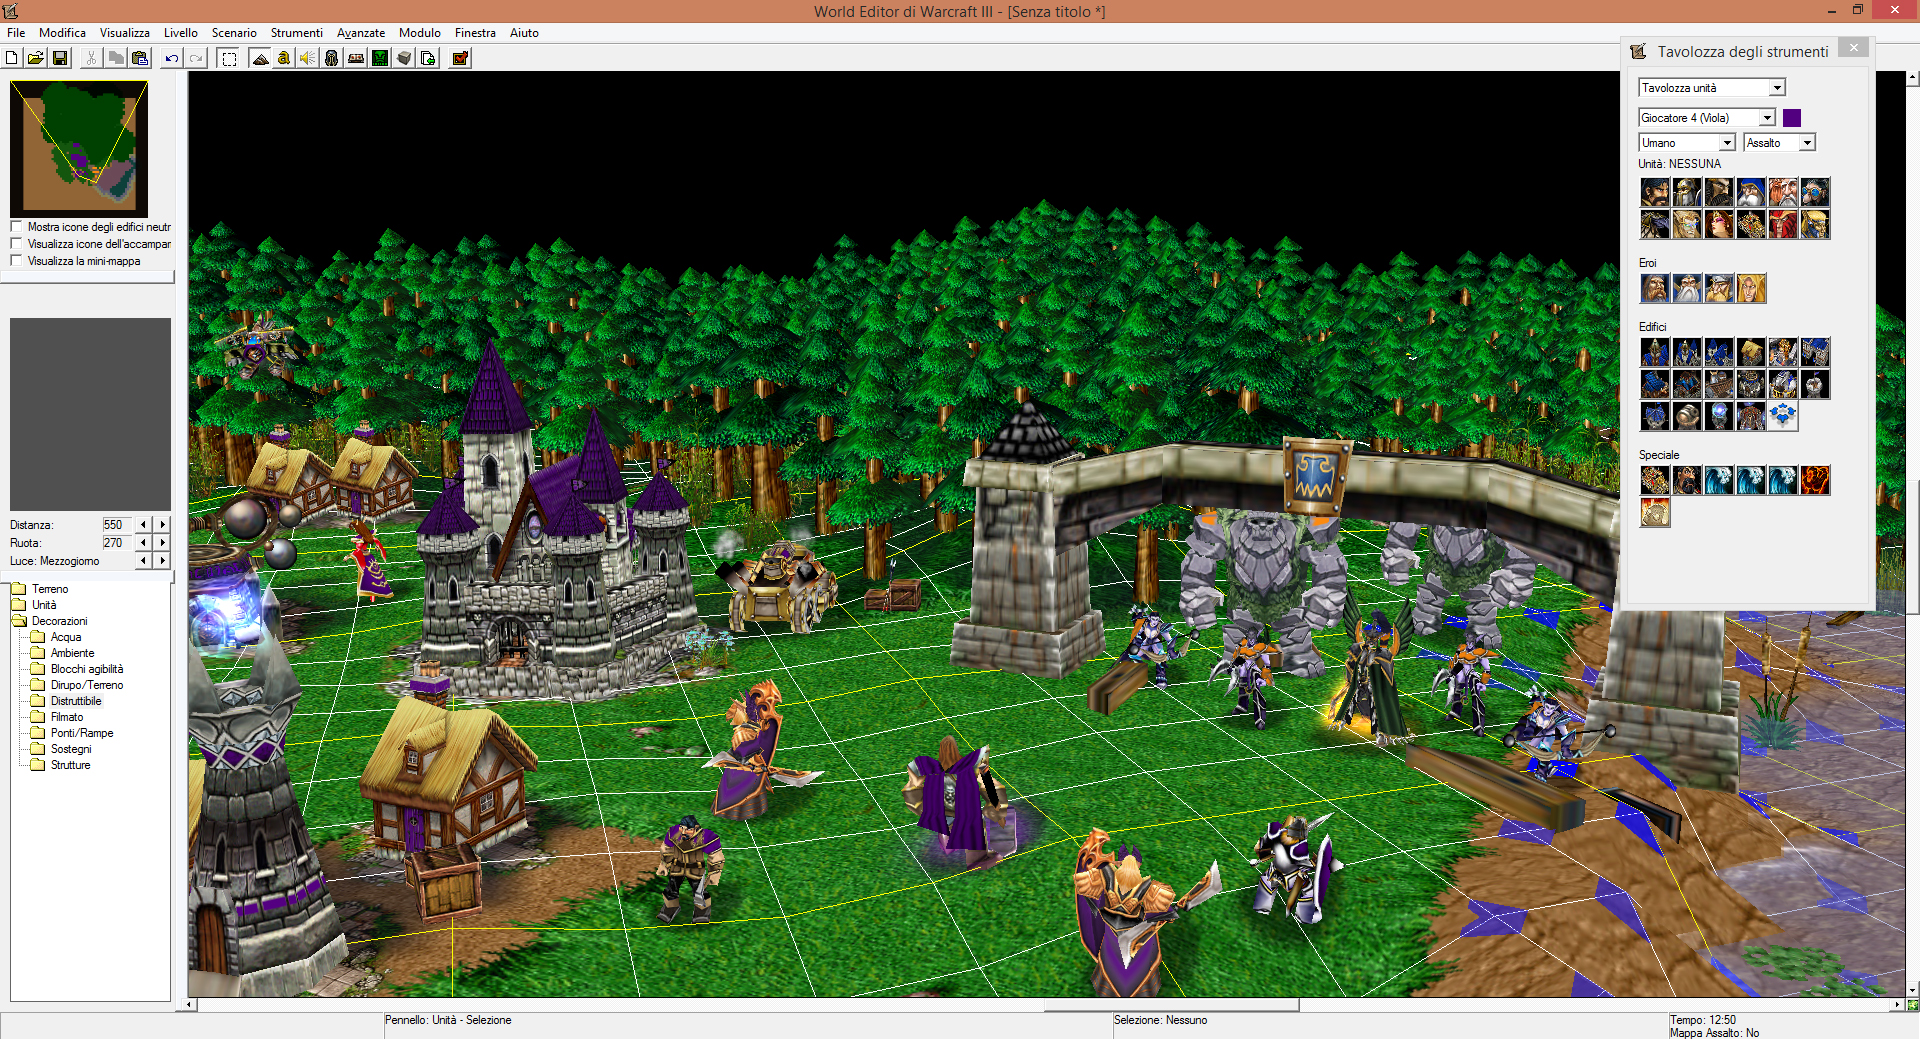
\includegraphics[width=.8\textwidth]{img/intro/World_Editor_di_Warcraft_III.jpg}
        \caption{Editor de mapas do \alert{Warcraft III}}
    \end{figure}
    \url{it.wikipedia.org/wiki/World_Editor_di_Warcraft_III}
\end{frame}

\begin{frame}{Contextualização}
    \begin{itemize}
        \item Conteúdo criado proceduralmente exige persistência do método(Algoritmo)
        \item Quanto maior o mundo virtual, tecnicamente mais tempo os jogadores irão explorar \cite{bevilacqua2009ferramenta}
    \end{itemize}
\end{frame}


\begin{frame}{Contextualização}
    \begin{figure}
		\centering
        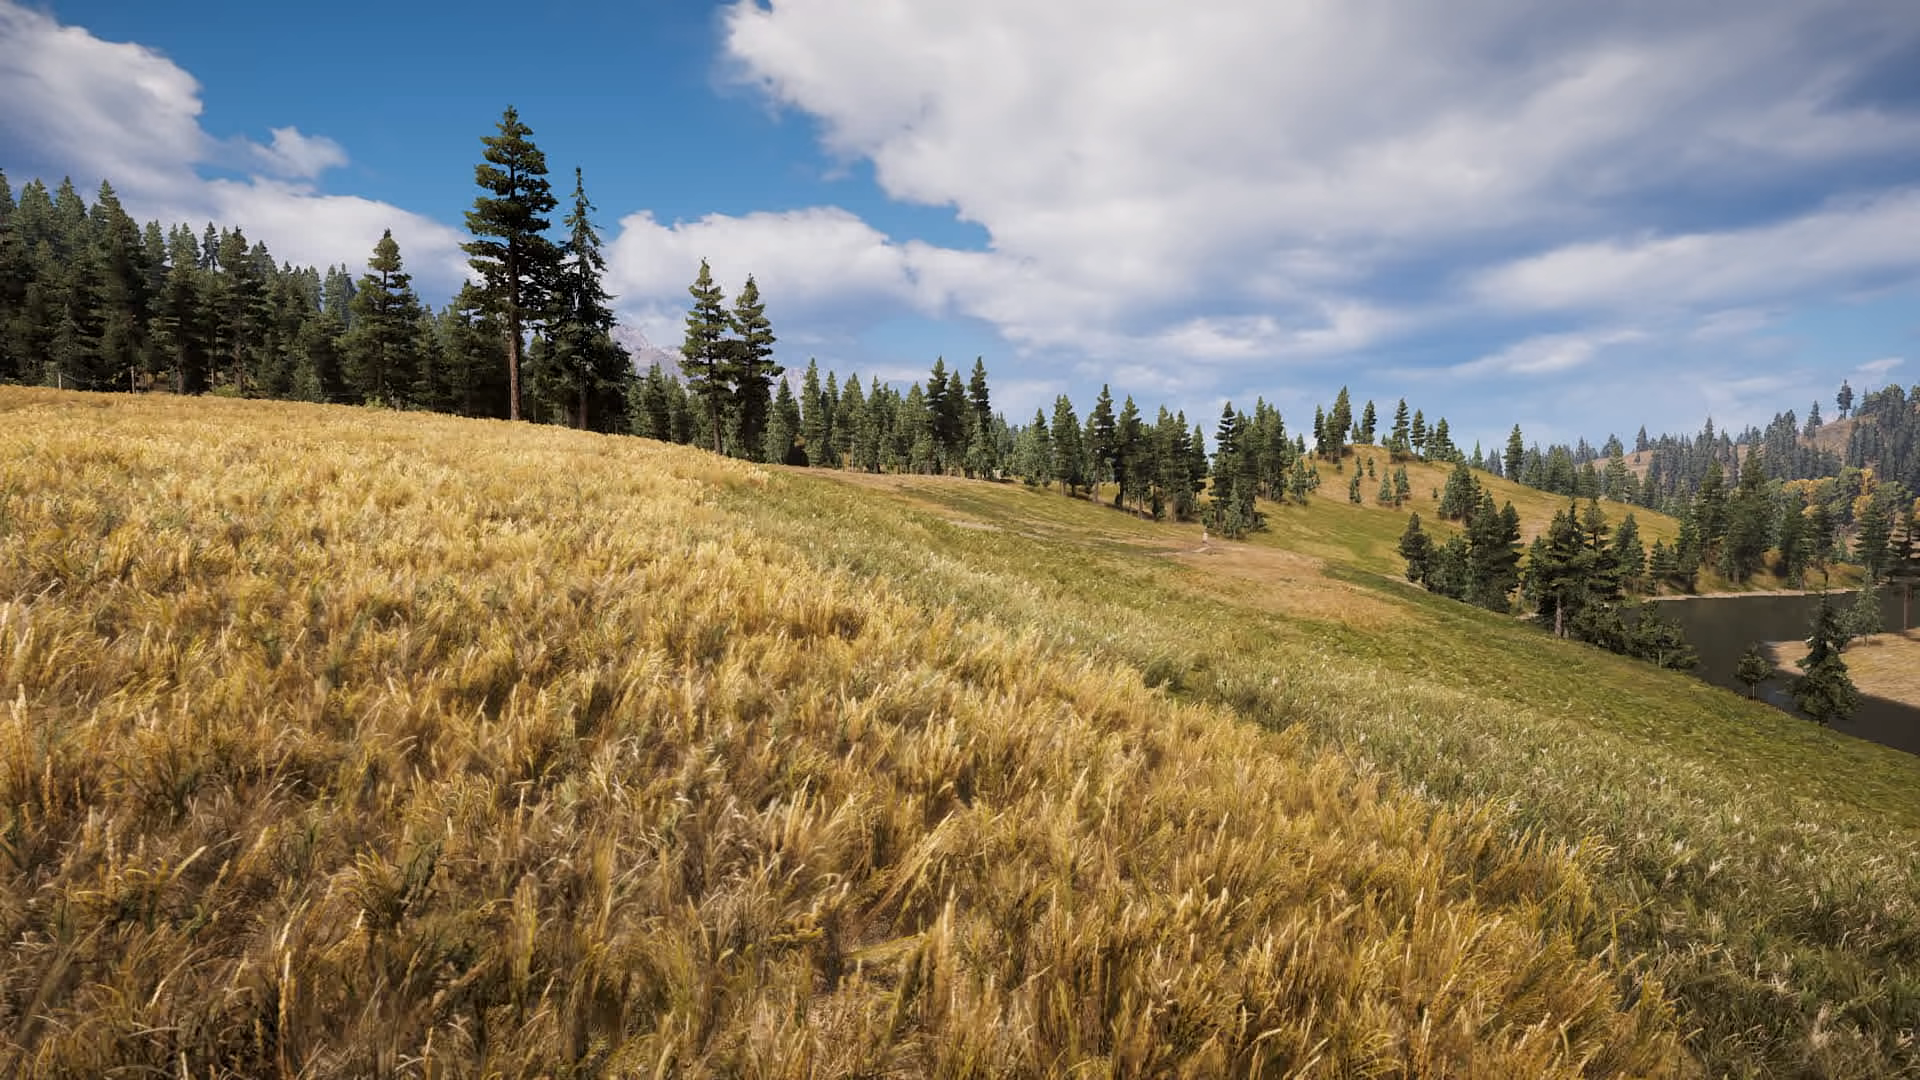
\includegraphics[width=.8\textwidth]{img/intro/fc5terrain.png}
        \caption{Mapa de \alert{Far Cry 5}, \cite{Carrier2018farcry5}}
    \end{figure}
\end{frame}

\begin{frame}{Contextualização}
    \begin{figure}
		\centering
        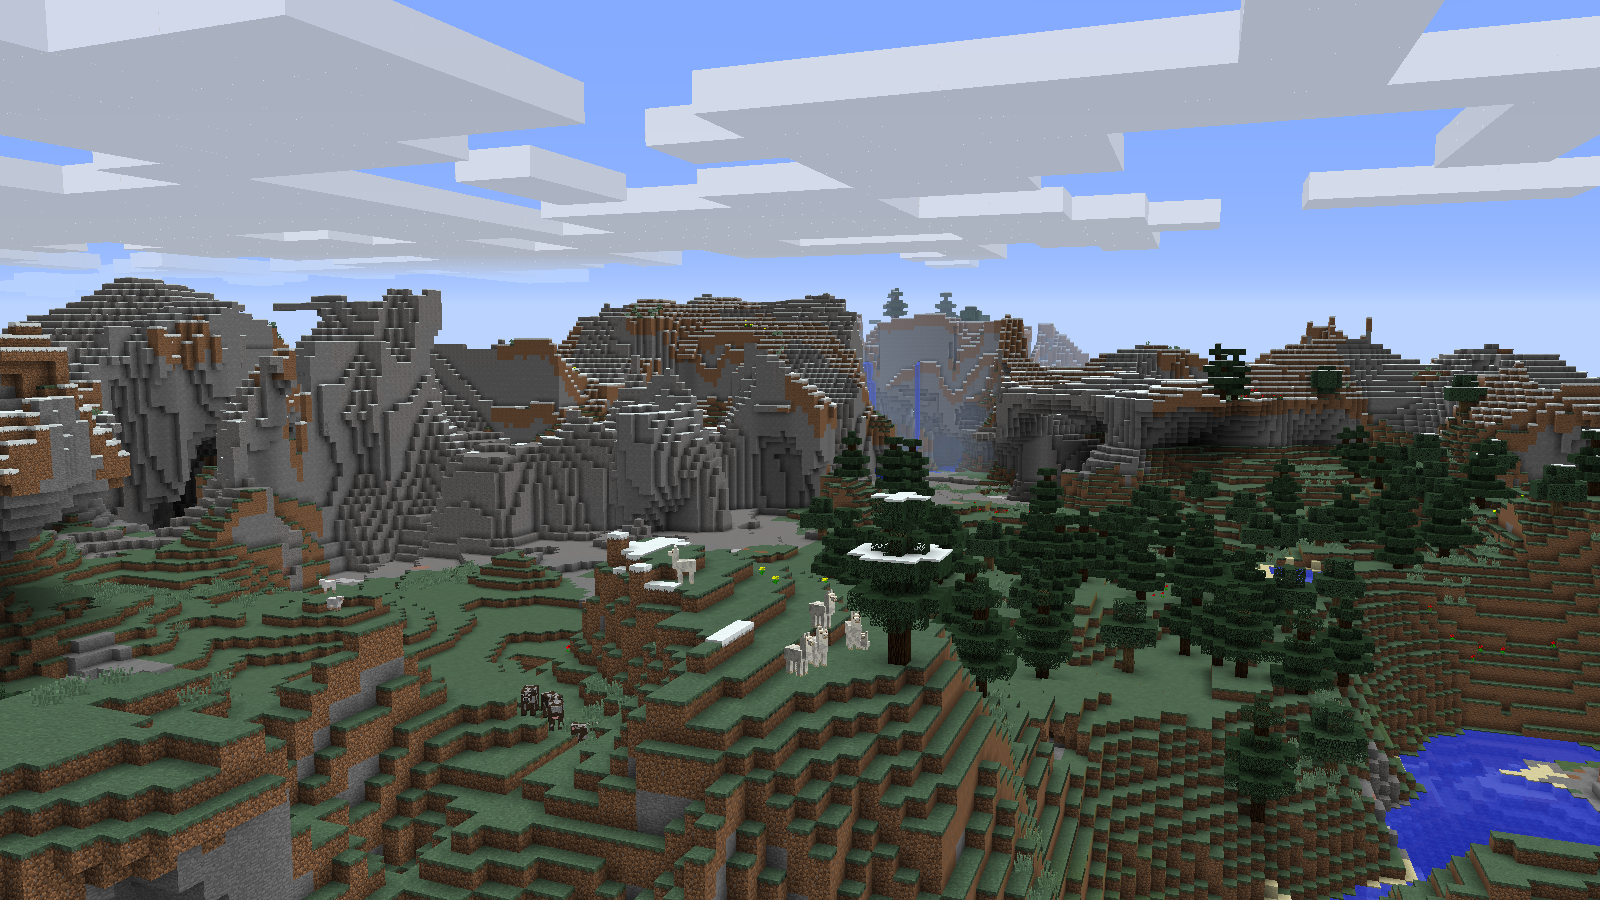
\includegraphics[width=.8\textwidth]{img/intro/mineExtremeHills.png}
        \caption{Mundo de \alert{Minecraft}}
    \end{figure}  
\end{frame}

\begin{frame}{Objetivo}
    \begin{itemize}
        \item Mostrar um método capaz de gerar um terreno para jogos
        \item Terrenos com relevos \alert{naturais}
    \end{itemize}
\end{frame}

\begin{frame}{Exemplo}
    \begin{figure}
		\centering
        \includegraphics[width=.8\textwidth]{img/intro/derby.jpg}
        \caption{Erosão Fractal}
    \end{figure}
    imagem de \url{paulbourke.net/fractals/googleearth/}
\end{frame}

\begin{frame}{Roteiro}
    \setbeamertemplate{section in toc}[sections numbered]
    \tableofcontents[hideallsubsections]
\end{frame}

\section{Requisitos}

% para algum ponto (x, z) precisa sempre gerar o mesmo y função (injetora) (consistência) (ser deterministico)
% (Variedade)
\begin{frame}{Requisitos}
    \begin{itemize}
        \item Determinismo, $ y = f(x, z) $
        \item \alert{Aleatoriedade}
    \end{itemize}
\end{frame}

\begin{frame}{Requisitos}
    \begin{figure}
		\centering
        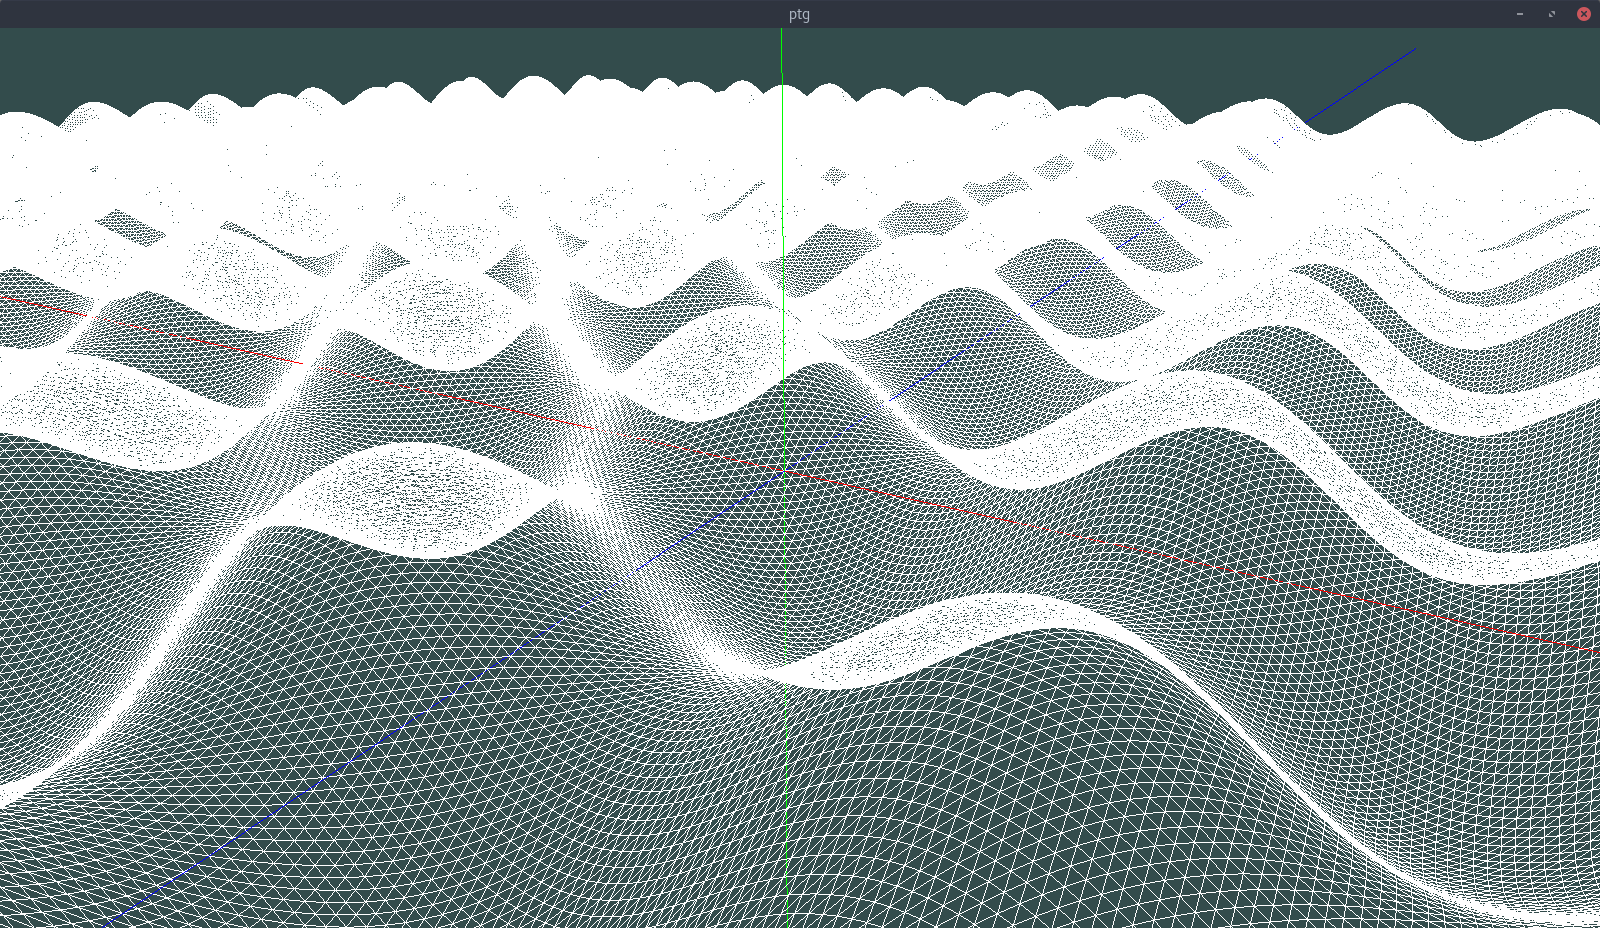
\includegraphics[width=.8\textwidth]{img/intro/sssins.png}
        \caption{$ y = sin(x) + sin(z) $}
    \end{figure}  
\end{frame}



\begin{frame}{Aproximação do Mundo Real}
    \begin{itemize}
        \item Mostrar um método capaz de gerar um terreno para jogos
        \item Terrenos com relevos \alert{naturais}
    \end{itemize}
\end{frame}
% O que tem em um terreno (padrões fractais)

\begin{frame}{Aproximação do Mundo Real}
    \begin{figure}
		\centering
        \includegraphics[width=.8\textwidth]{img/intro/derby.jpg}
        \caption{Erosão Fractal}
    \end{figure}
    imagem de \url{paulbourke.net/fractals/googleearth/}
\end{frame}

\section{Como é feito?}

% Juntar requisitos
% O que tem em um terreno (padrões fractais)
% para algum ponto (x, z) precisa sempre gerar o mesmo y função (injetora) 
% (consistência)


% O que é perlin Noise?
% Carregar apenas área perto do jogador
% Mostrar o que é tesselation

% \begin{frame}{Figura Teste}
%   \begin{figure}
% 		\centering
%         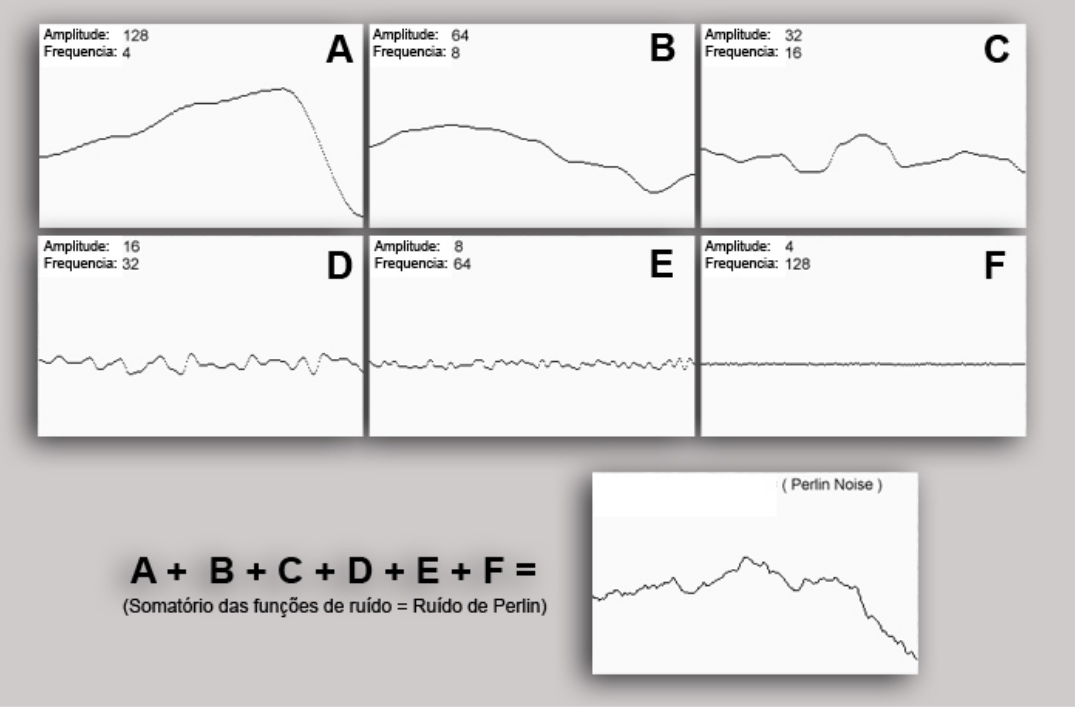
\includegraphics[width=.7\textwidth]{img/perlin1d.png}
%         \caption{Ruído de Perlin em uma dimensão.}
%   \end{figure}
% \end{frame}

\begin{frame}{Perlin Noise octaves}
    \begin{equation*}
        \begin{split} 
            \visible<+->{max & = \lim_{n\to \infty} 2^{-n} (2^{n +1}-1) \\}
            \visible<+->{& = 2}
        \end{split}
    \end{equation*}
\end{frame}

%mostrar dimenções e manipulações do ruido

%limitações, é realmente infinito?


\section{Contribuições da UFFS}

% Trabalho da Gabrielle
\begin{frame}{Geração Procedural de Cânions Baseado em Ruído de Perlin}
  \begin{itemize}
        \item A partir de uma classificação de características de cânions;
        \item As características mais comuns foram selecionadas.
    \end{itemize}
\end{frame}

\begin{frame}{Geração Procedural de Cânions Baseado em Ruído de Perlin}
  \begin{figure}
		\centering
        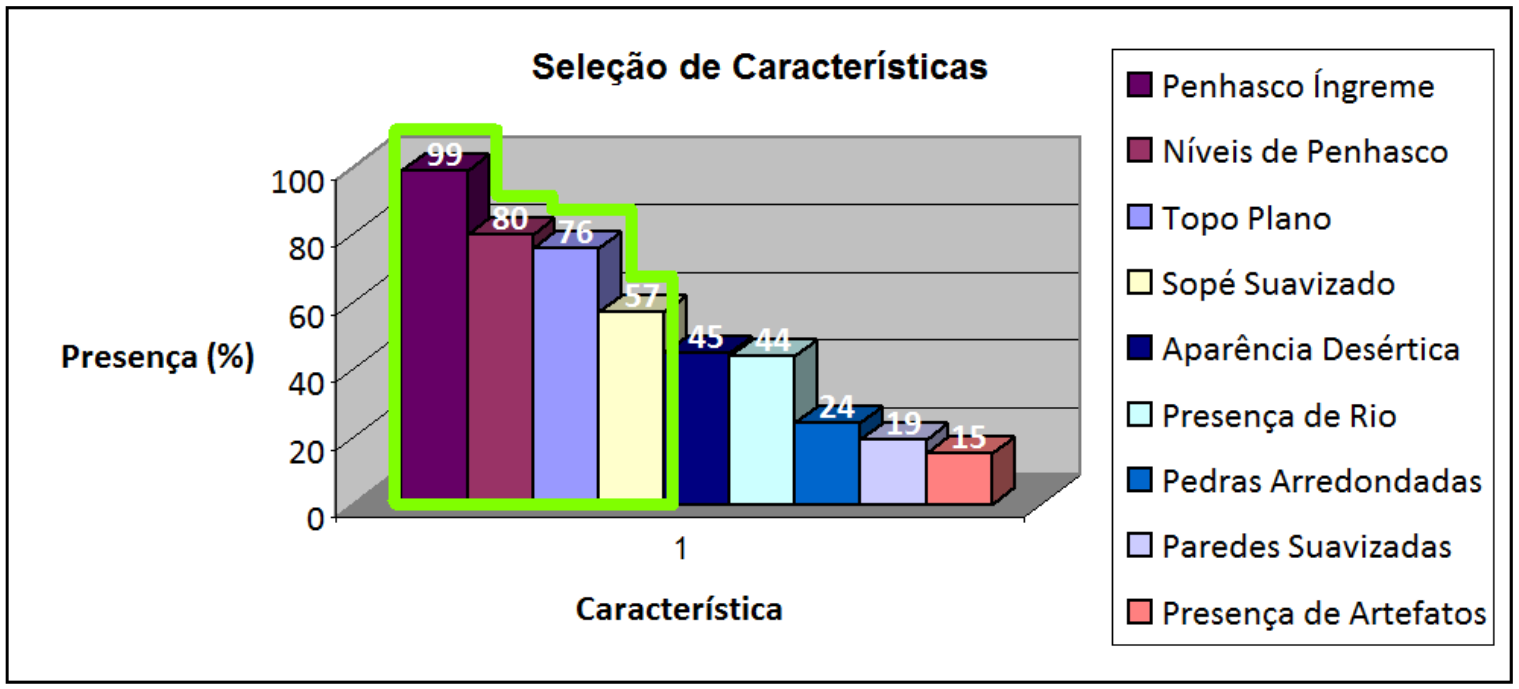
\includegraphics[width=.8\textwidth]{img/uffs/caract.png}
        \caption{Frequência de características nos cânions 
        \cite{gabrielle2016canion}.}
  \end{figure}
\end{frame}

\begin{frame}{Geração Procedural de Cânions Baseado em Ruído de Perlin}
  \begin{figure}
		\centering
        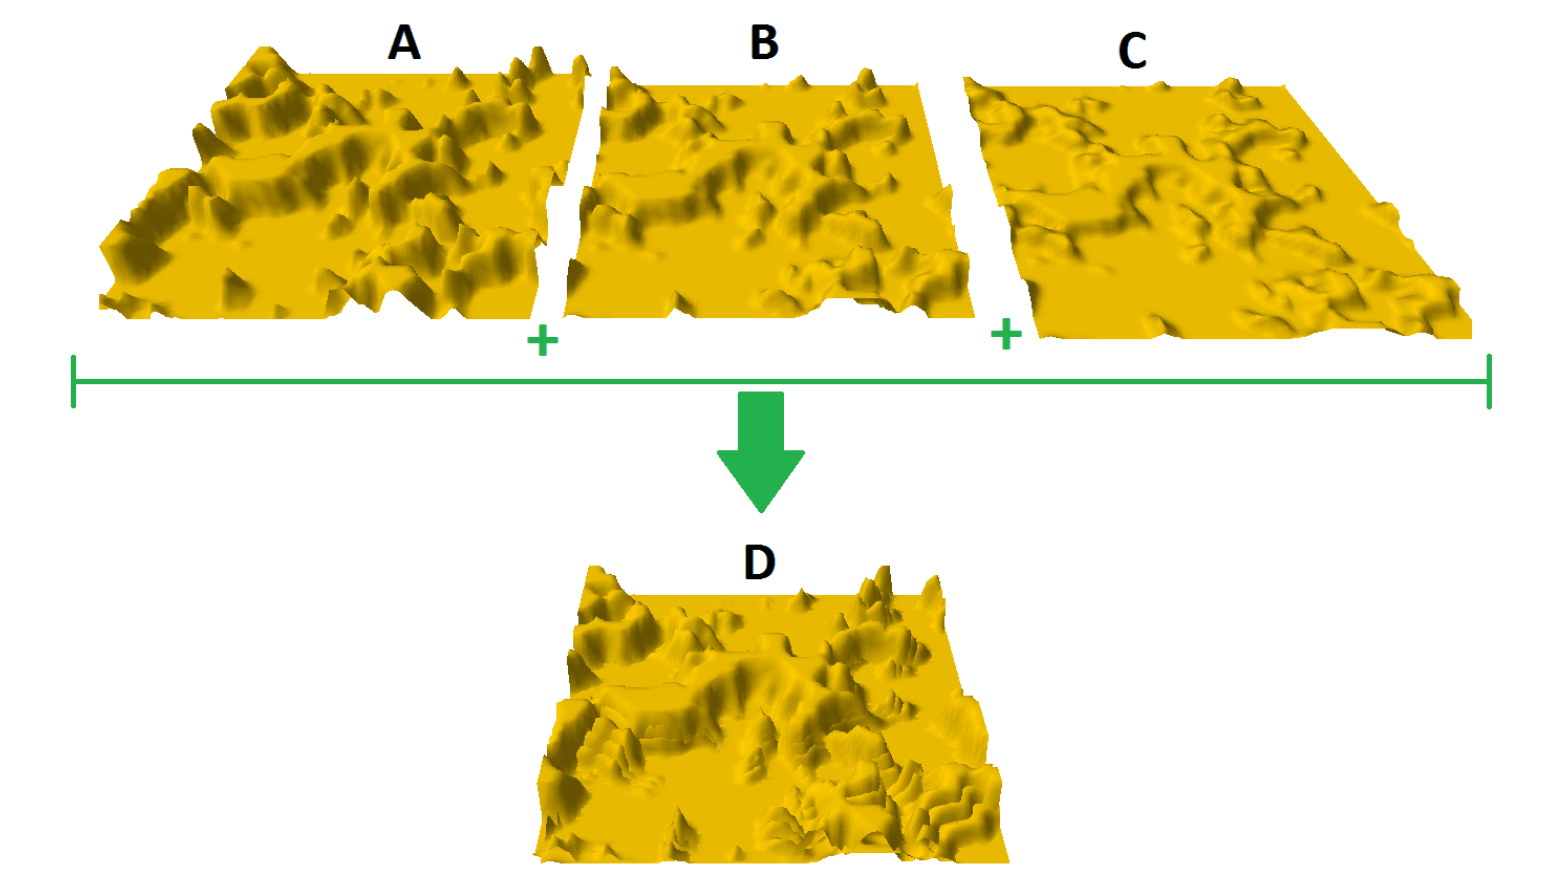
\includegraphics[width=.8\textwidth]{img/uffs/gabrielleDev.png}
        \caption{Soma das camadas para gerar Cânions}
  \end{figure}
\end{frame}

\begin{frame}{Geração Procedural de Cânions Baseado em Ruído de Perlin}
  \begin{figure}
		\centering
        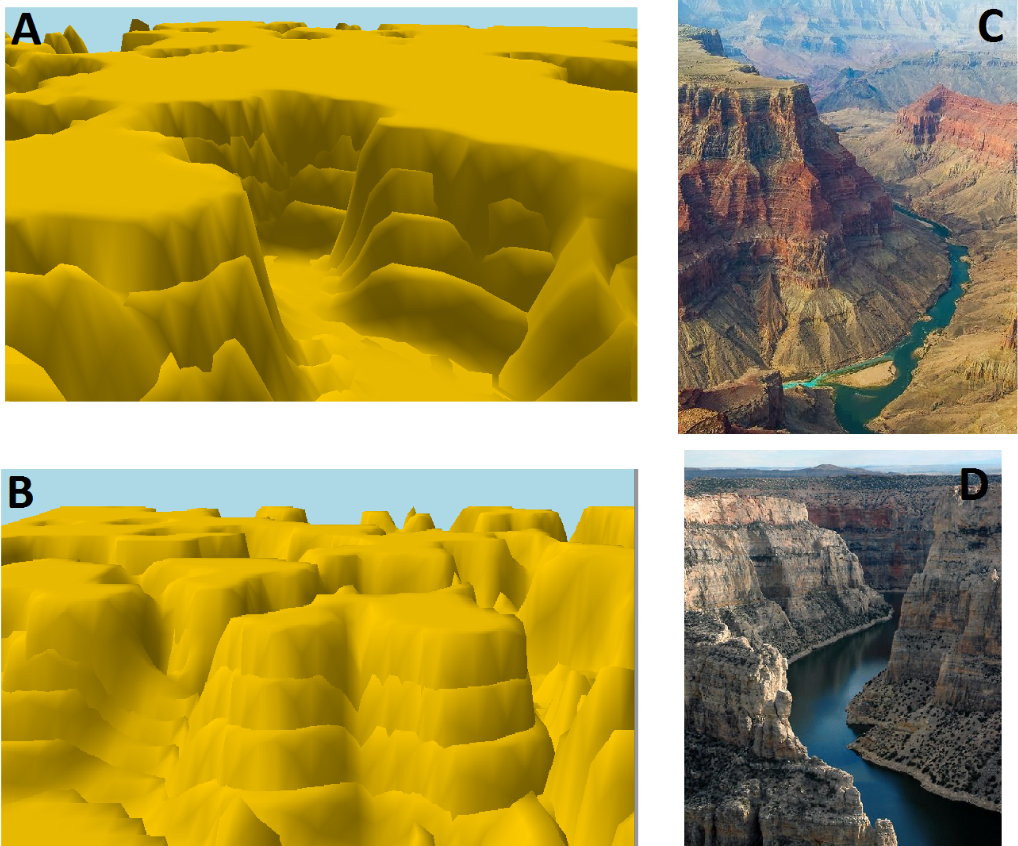
\includegraphics[width=.65\textwidth]{img/uffs/gabrielleResultado.png}
        \caption{Resultado Final}
  \end{figure}
\end{frame}


% Meu trabalho
\begin{frame}{Geração de Terrenos com Biomas Distintos para Jogos}
    \begin{itemize}
        \item Implementação de relevo para 5 \alert{Biomas}
            \begin{itemize}
                \item Planícies
                \item Montanhas
                \item Vales
                \item Deserto
                \item Cânions
            \end{itemize}
        \item Distribuição dos Biomas
        \item Suavização das fronteiras
    \end{itemize}
\end{frame}

\begin{frame}{Geração de Terrenos com Biomas Distintos para Jogos}
    \begin{figure}
		\centering
        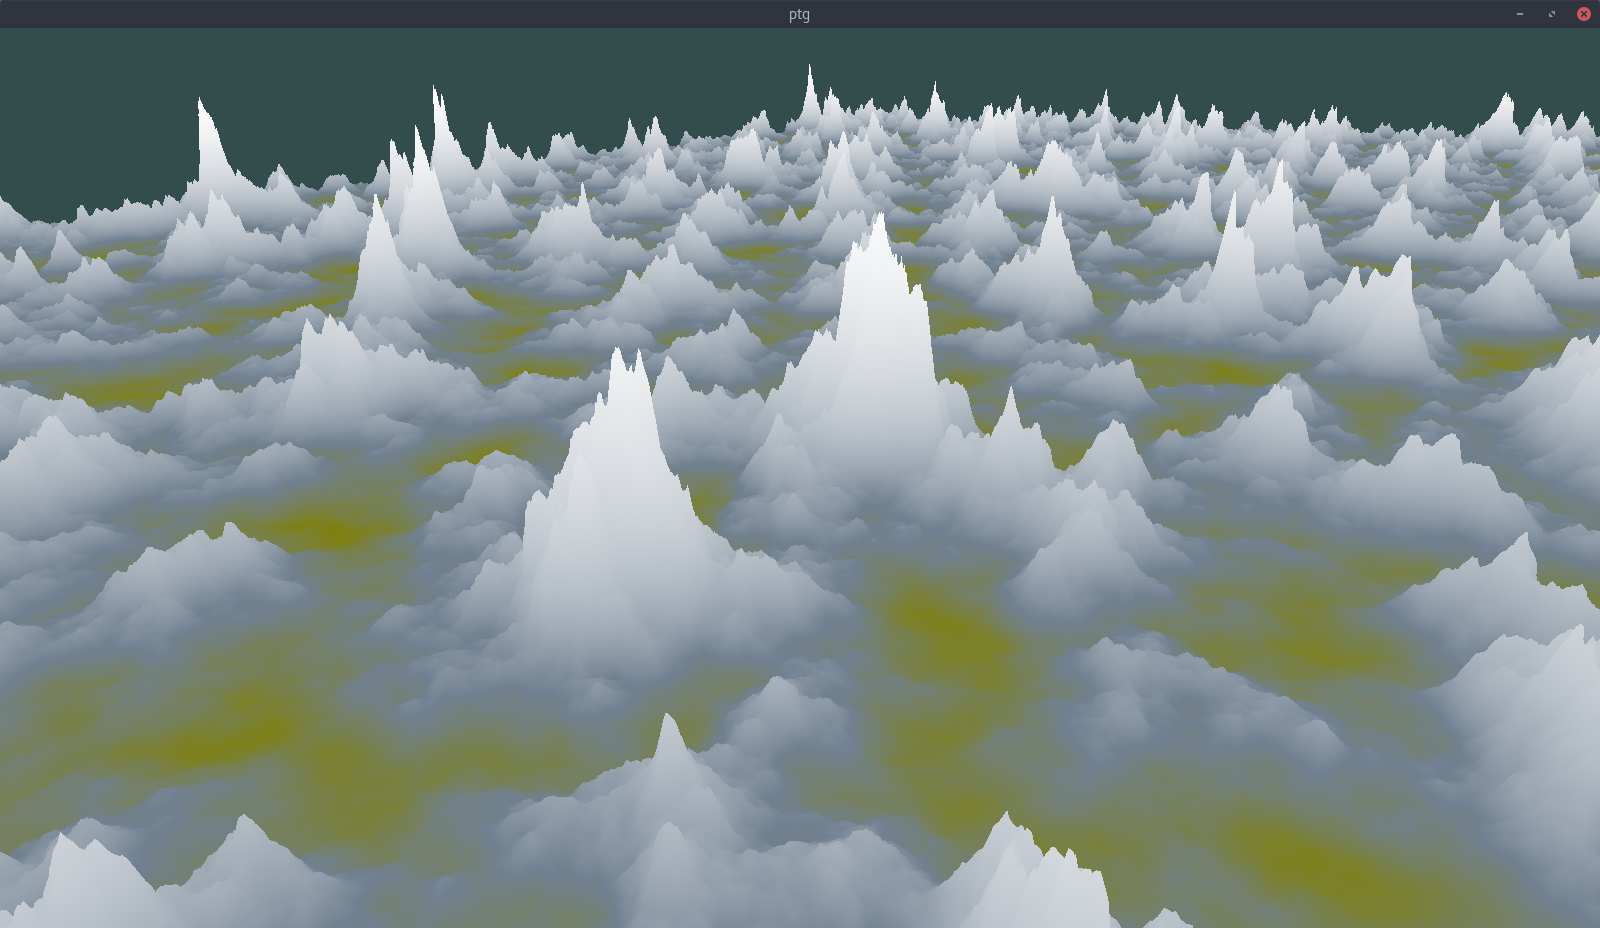
\includegraphics[width=.8\textwidth]{img/uffs/bssMontains.png}
        \caption{Montanhas, $h = 1.5^{h'\cdot 7}\cdot 5$}
    \end{figure}
\end{frame}

\begin{frame}{Geração de Terrenos com Biomas Distintos para Jogos}
    \begin{figure}
		\centering
        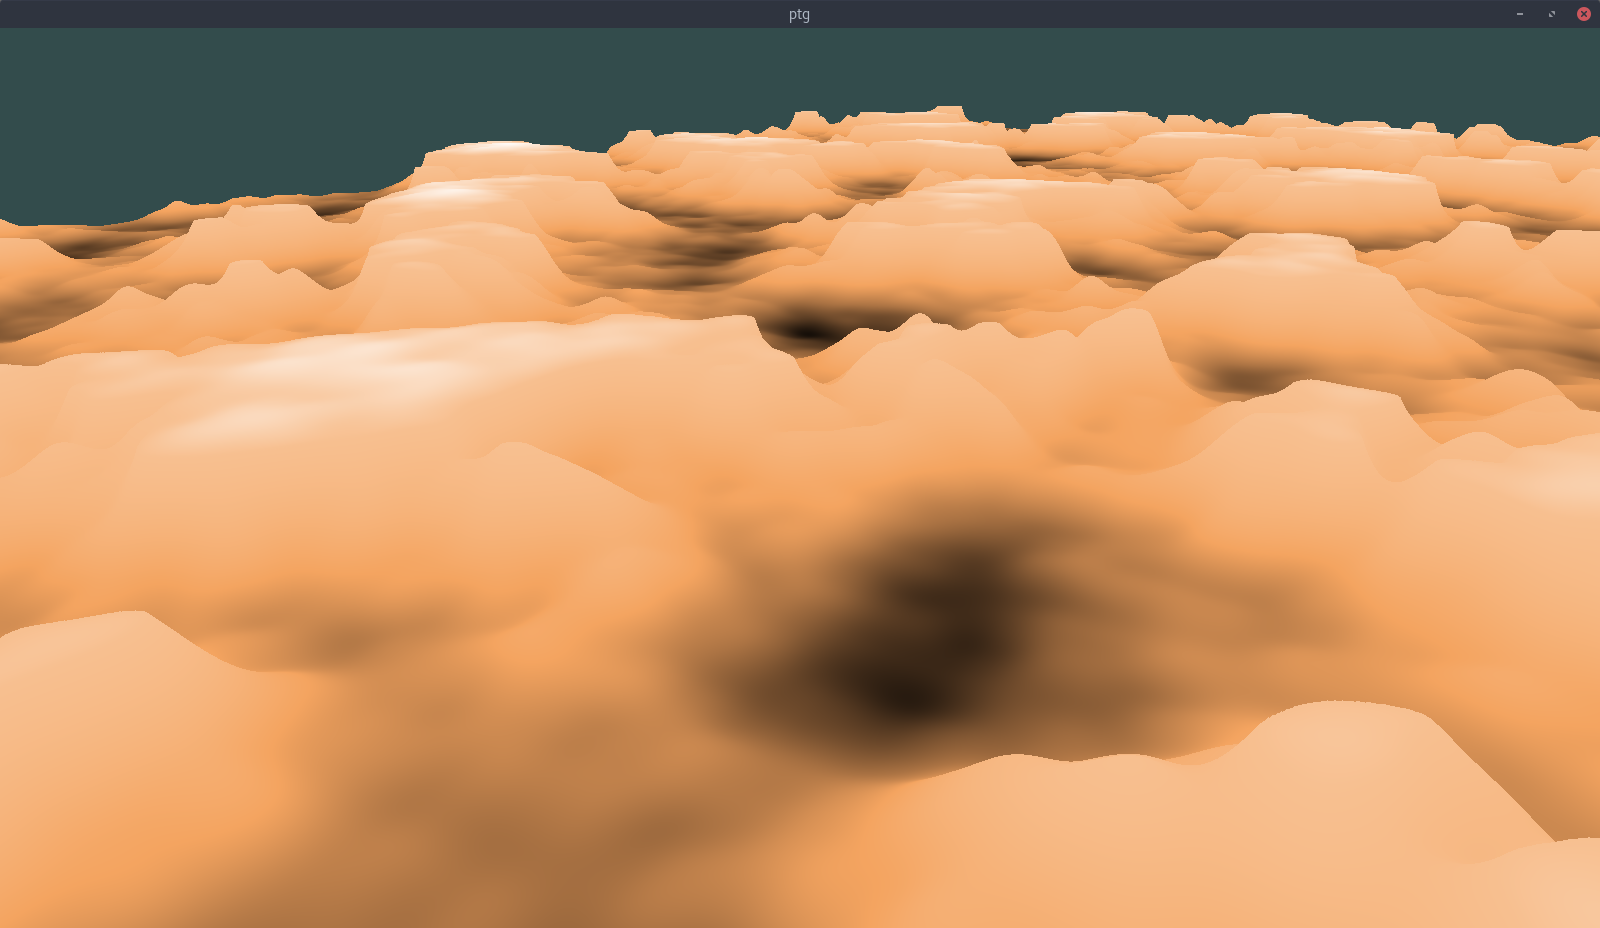
\includegraphics[width=.8\textwidth]{img/uffs/bssCanyons.png}
        \caption{Cânions, $h = (1.5^{clamp(h', -0.3, 0.3) \cdot 14}) \cdot 5 + h' \cdot 8$}
    \end{figure}
\end{frame}

\begin{frame}{Geração de Terrenos com Biomas Distintos para Jogos}
    \begin{figure}
		\centering
        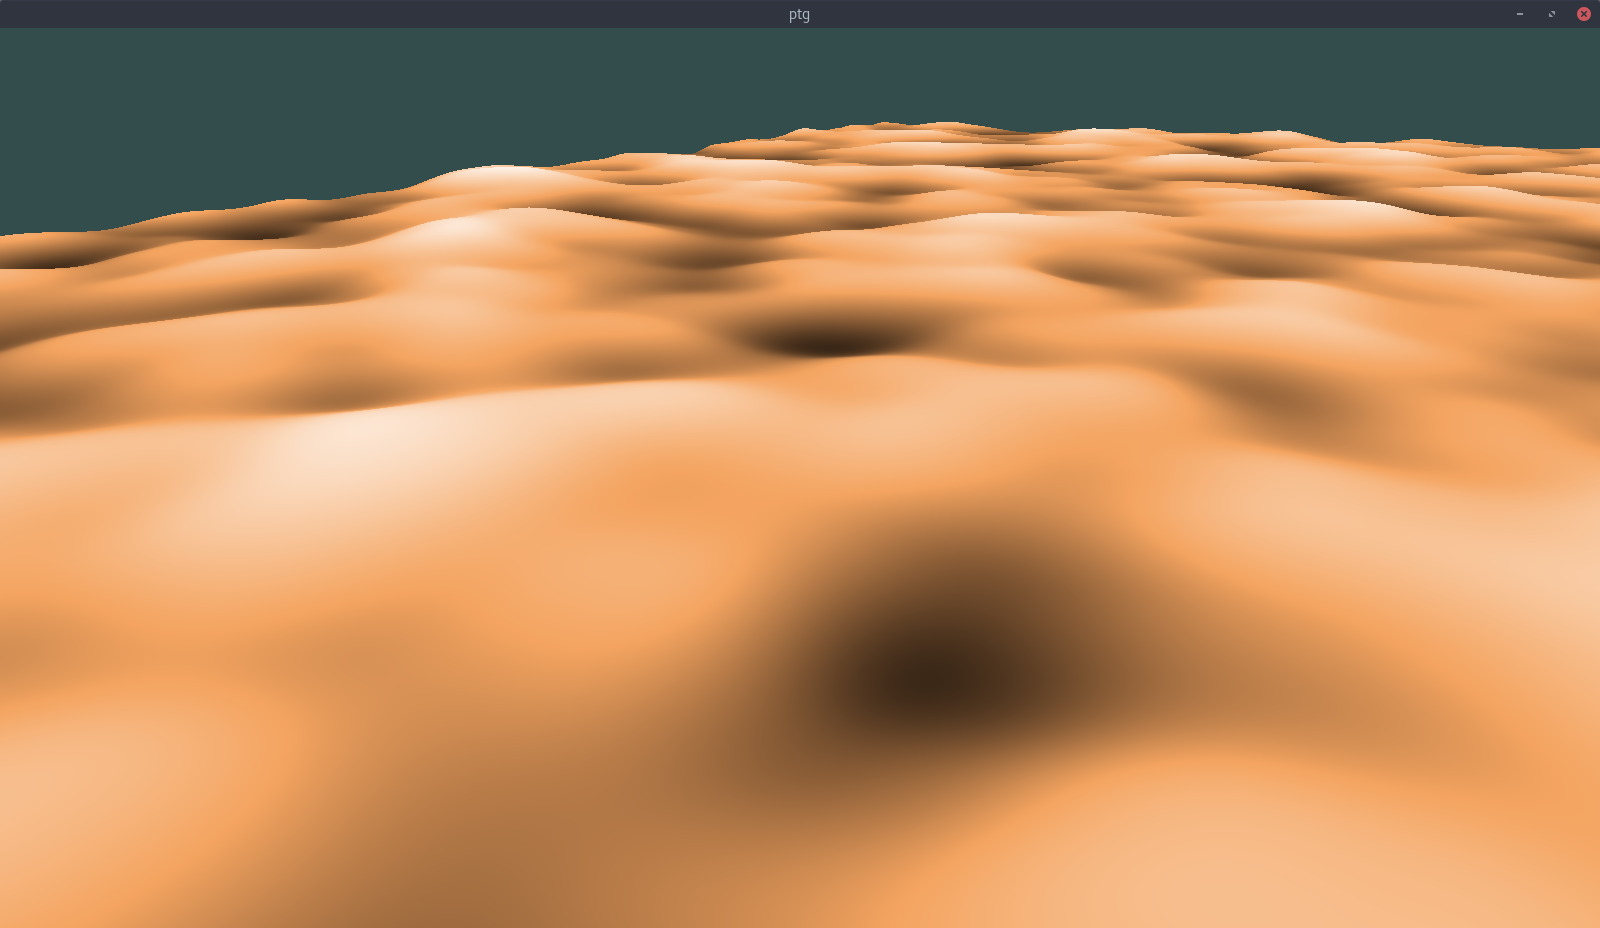
\includegraphics[width=.8\textwidth]{img/uffs/bssDesert.png}
        \caption{Deserto, $h = h' \cdot 16$}
    \end{figure}
\end{frame}

\begin{frame}{Geração de Terrenos com Biomas Distintos para Jogos}
    \begin{figure}
		\centering
        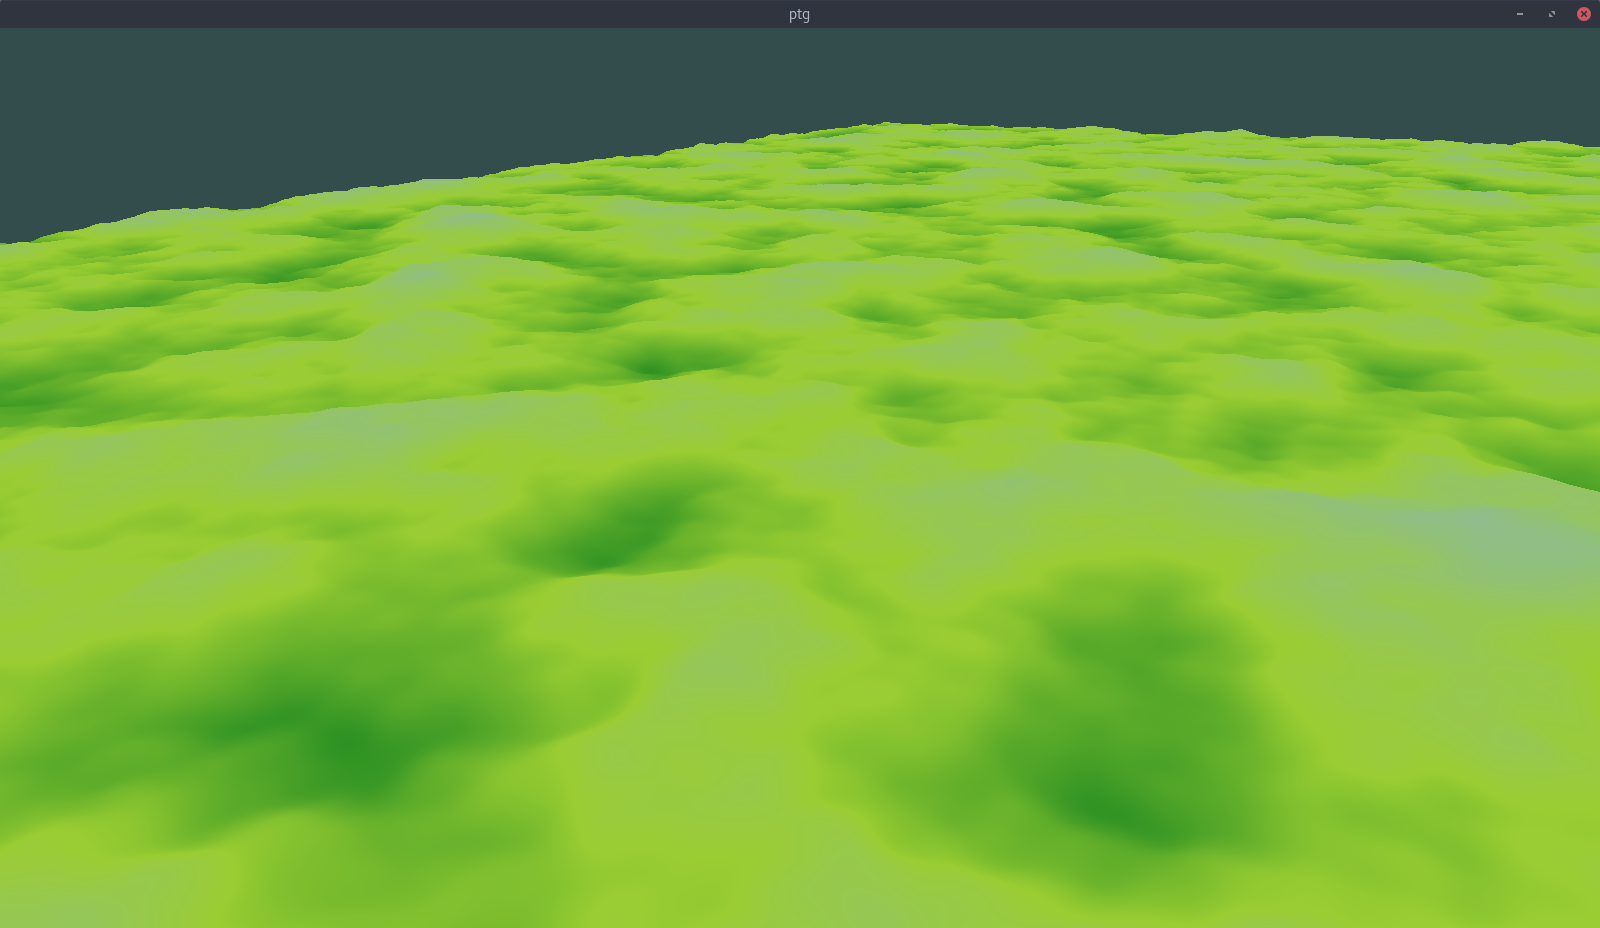
\includegraphics[width=.8\textwidth]{img/uffs/bssPlains.png}
        \caption{Planícies, $h = h' \cdot 10$}
    \end{figure}
\end{frame}

\begin{frame}{Geração de Terrenos com Biomas Distintos para Jogos}
    \begin{figure}
		\centering
        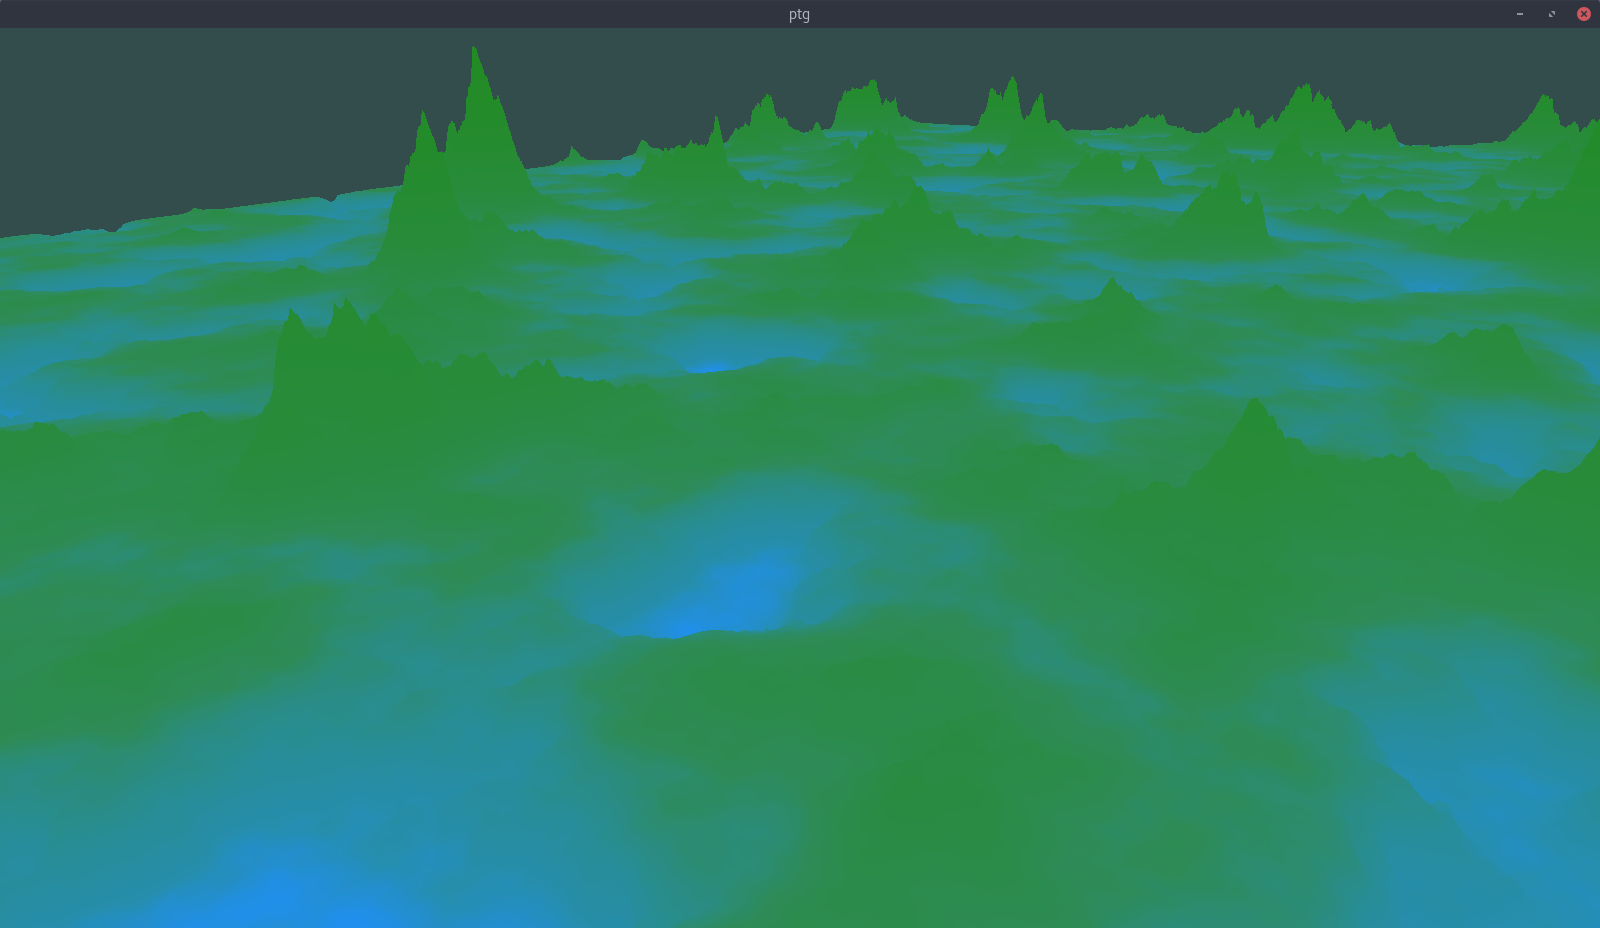
\includegraphics[width=.8\textwidth]{img/uffs/bssValley.png}
        \caption{Vales, $h = ($clamp($h', -0.5, 1.0$)$\cdot 5)^{3}$}
    \end{figure}
\end{frame}

\begin{frame}{Geração de Terrenos com Biomas Distintos para Jogos}
    \begin{figure}
		\centering
        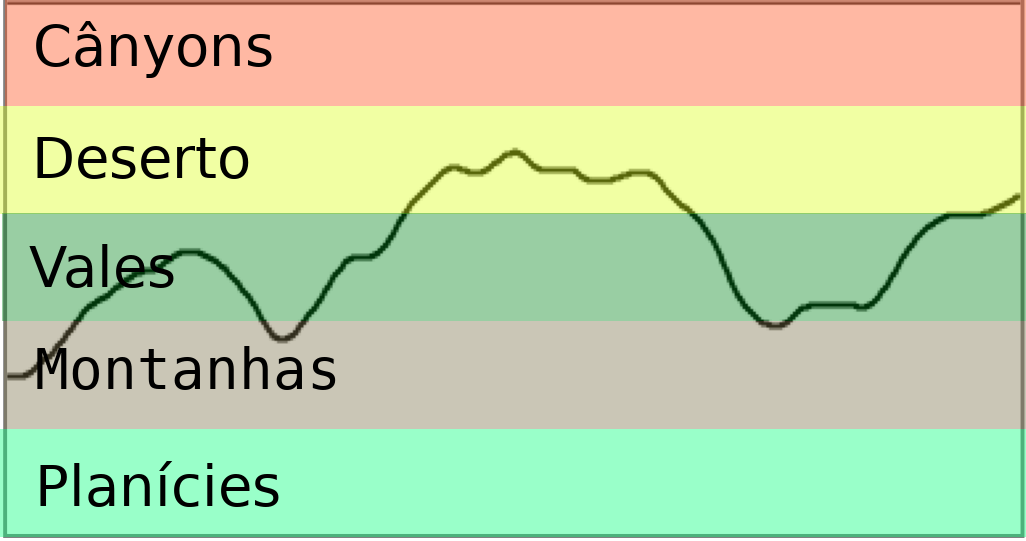
\includegraphics[width=.8\textwidth]{img/uffs/biomesdistnoise.png}
        \caption{Distribuição de Biomas}
    \end{figure}
\end{frame}

\begin{frame}{Geração de Terrenos com Biomas Distintos para Jogos}
    \begin{figure}
		\centering
        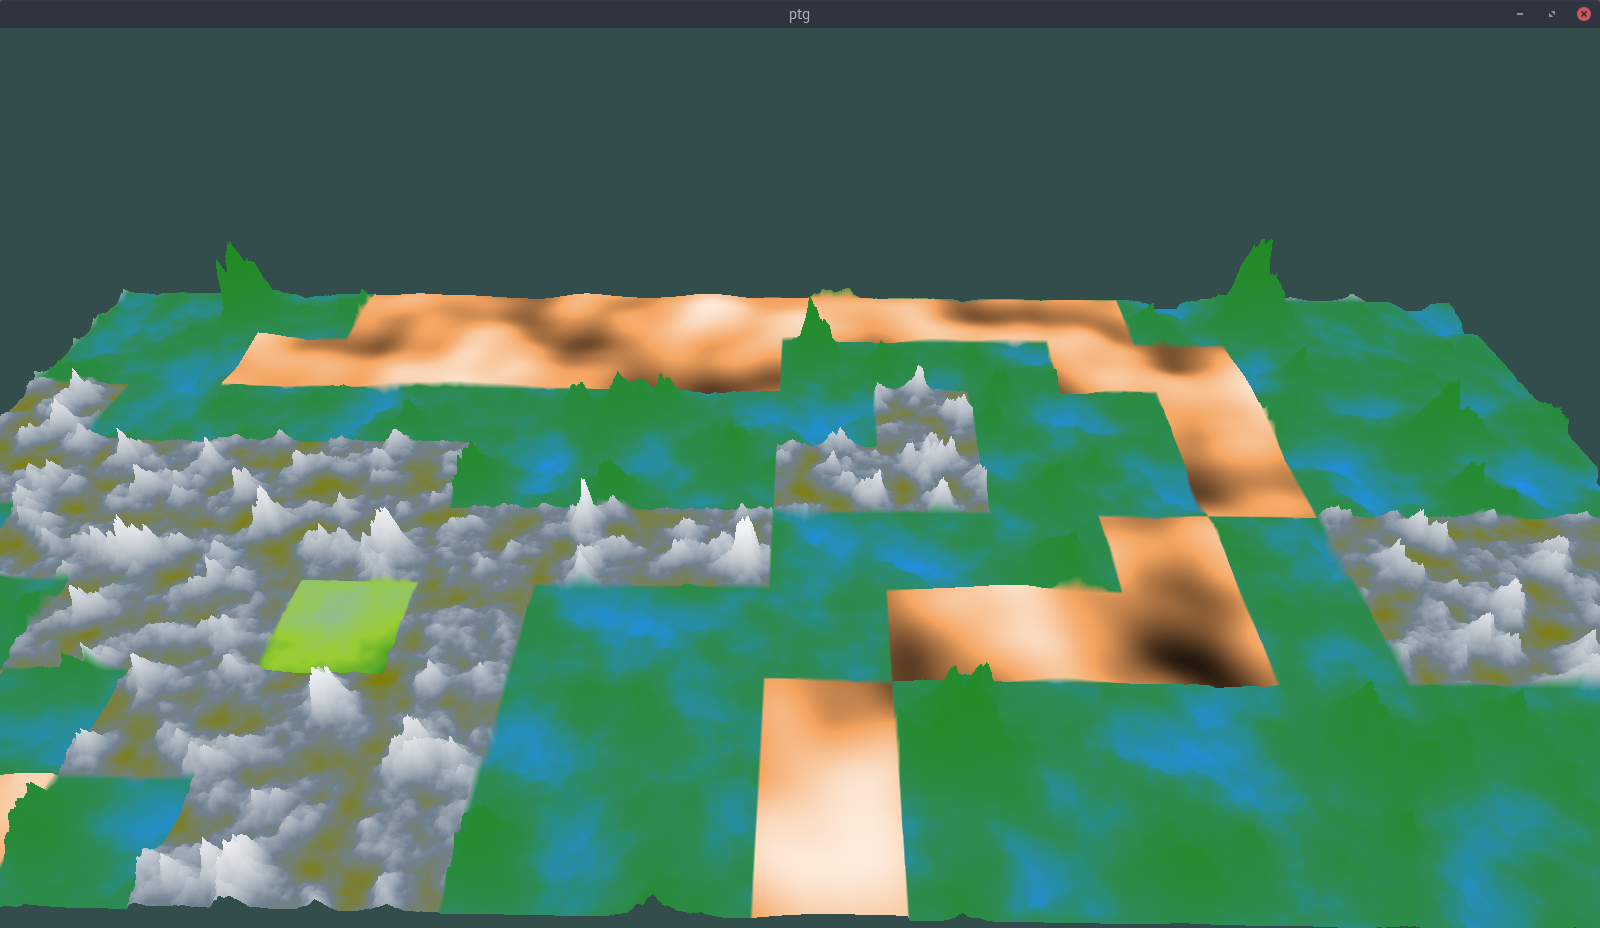
\includegraphics[width=.8\textwidth]{img/uffs/256f4.png}
        \caption{Distribuição de Biomas}
    \end{figure}
\end{frame}

\begin{frame}{Geração de Terrenos com Biomas Distintos para Jogos}
  \begin{figure}
		\centering
        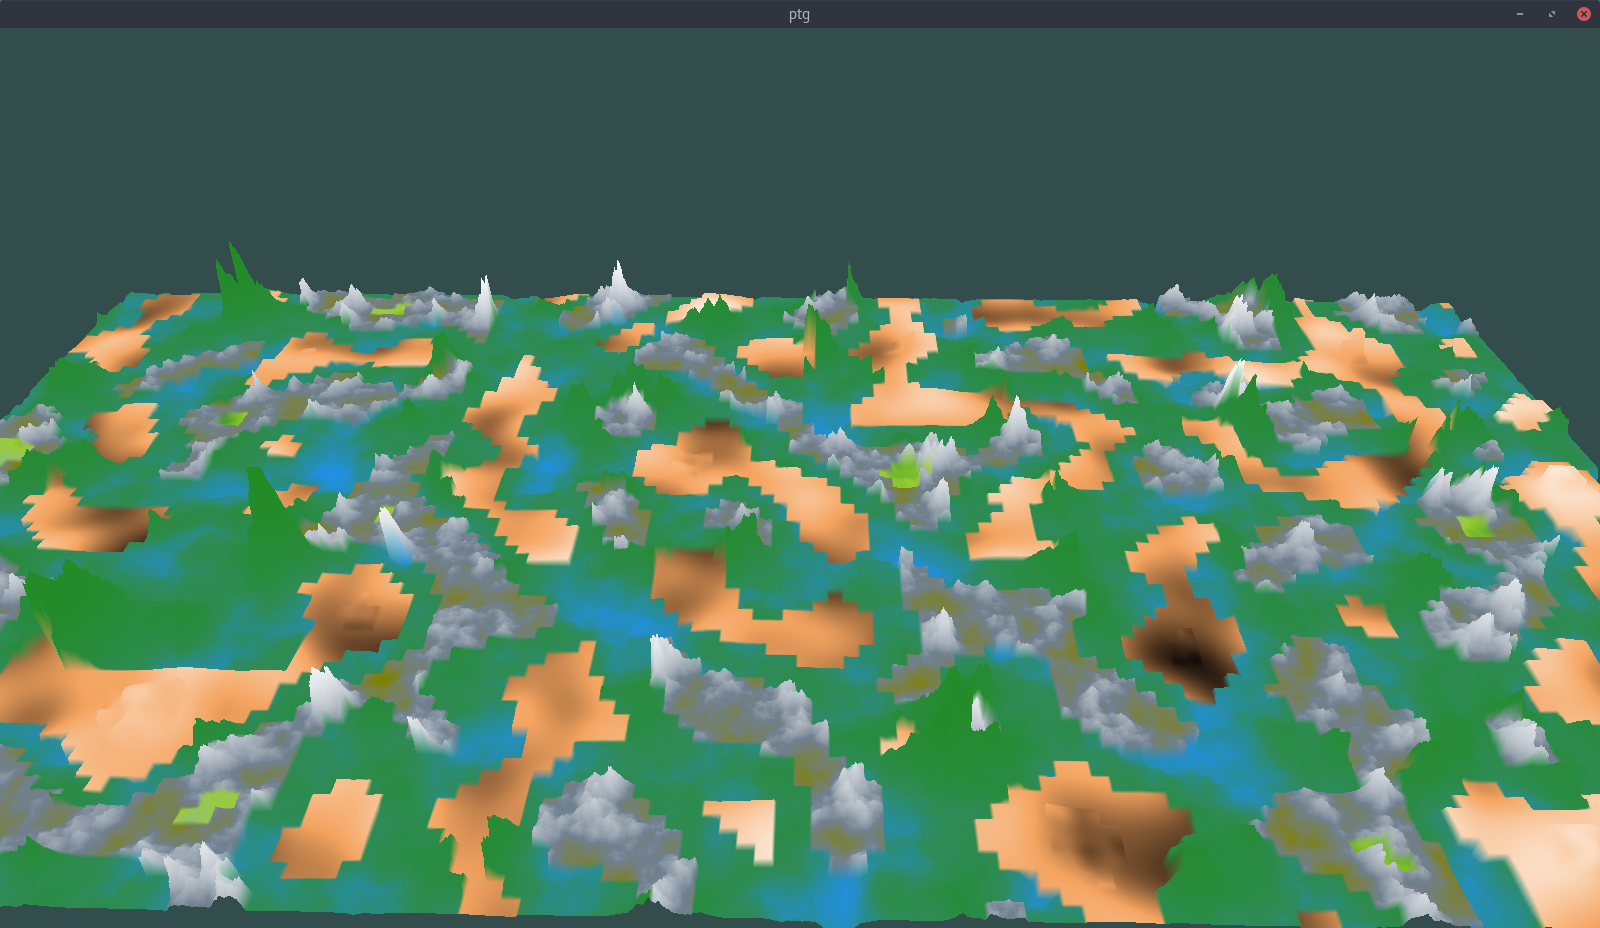
\includegraphics[width=.8\textwidth]{img/uffs/8b32.png}
        \caption{Frequência de Biomas = 8}
  \end{figure}
\end{frame}

\begin{frame}{Geração de Terrenos com Biomas Distintos para Jogos}
  \begin{figure}
		\centering
        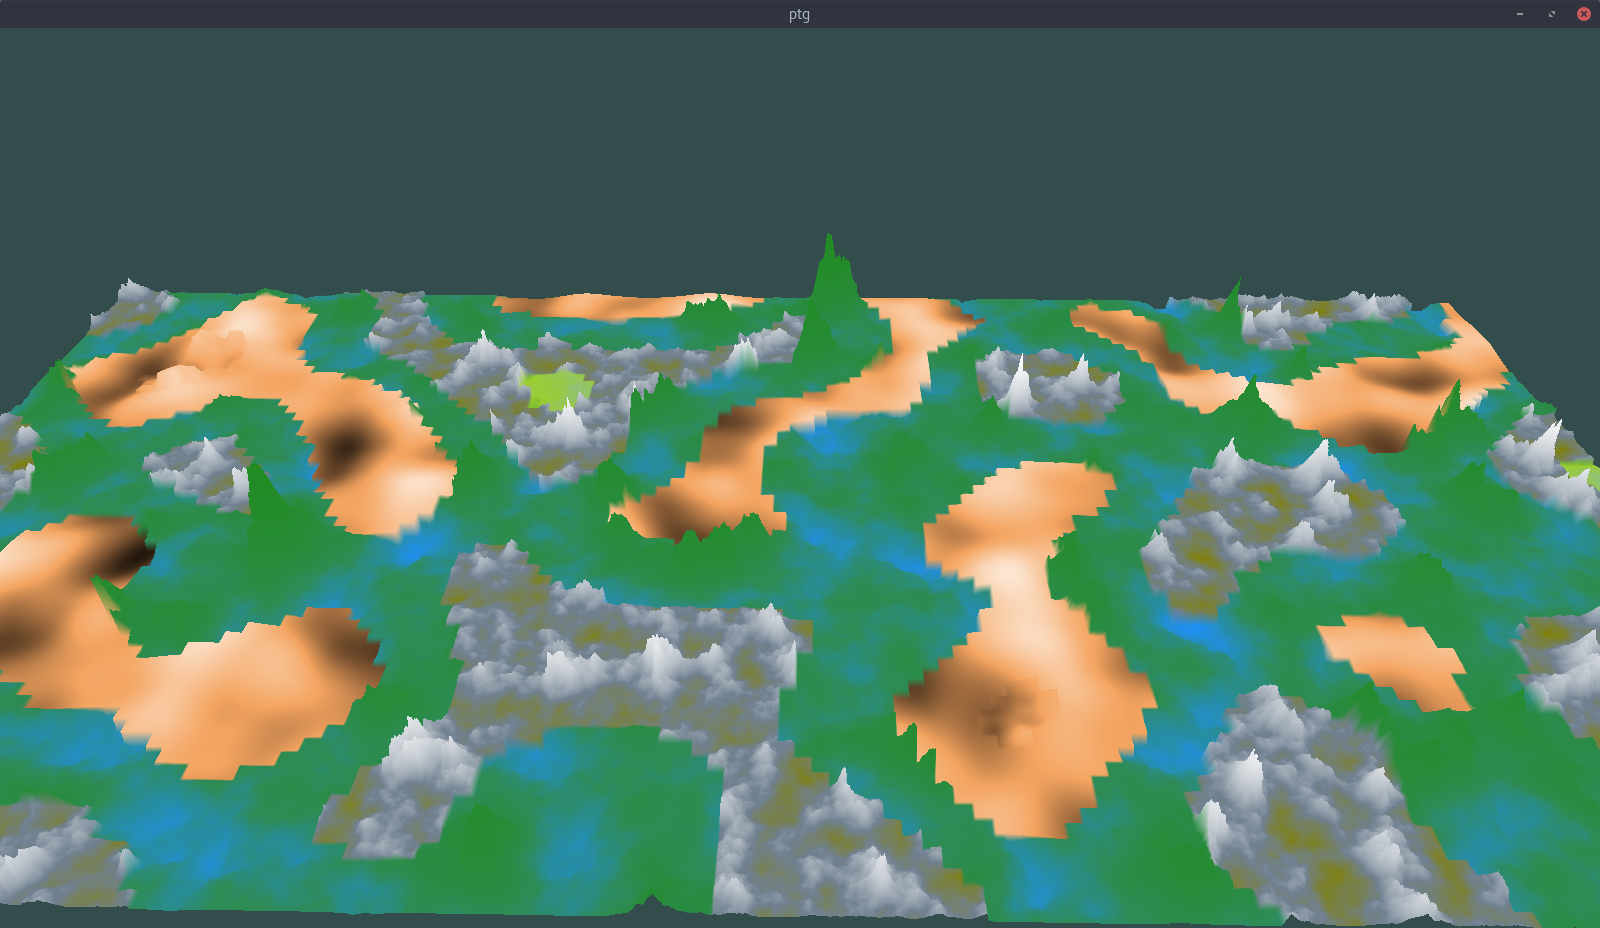
\includegraphics[width=.8\textwidth]{img/uffs/16b32.png}
        \caption{Frequência de Biomas = 16}
  \end{figure}
\end{frame}

\begin{frame}{Geração de Terrenos com Biomas Distintos para Jogos}
  \begin{figure}
		\centering
        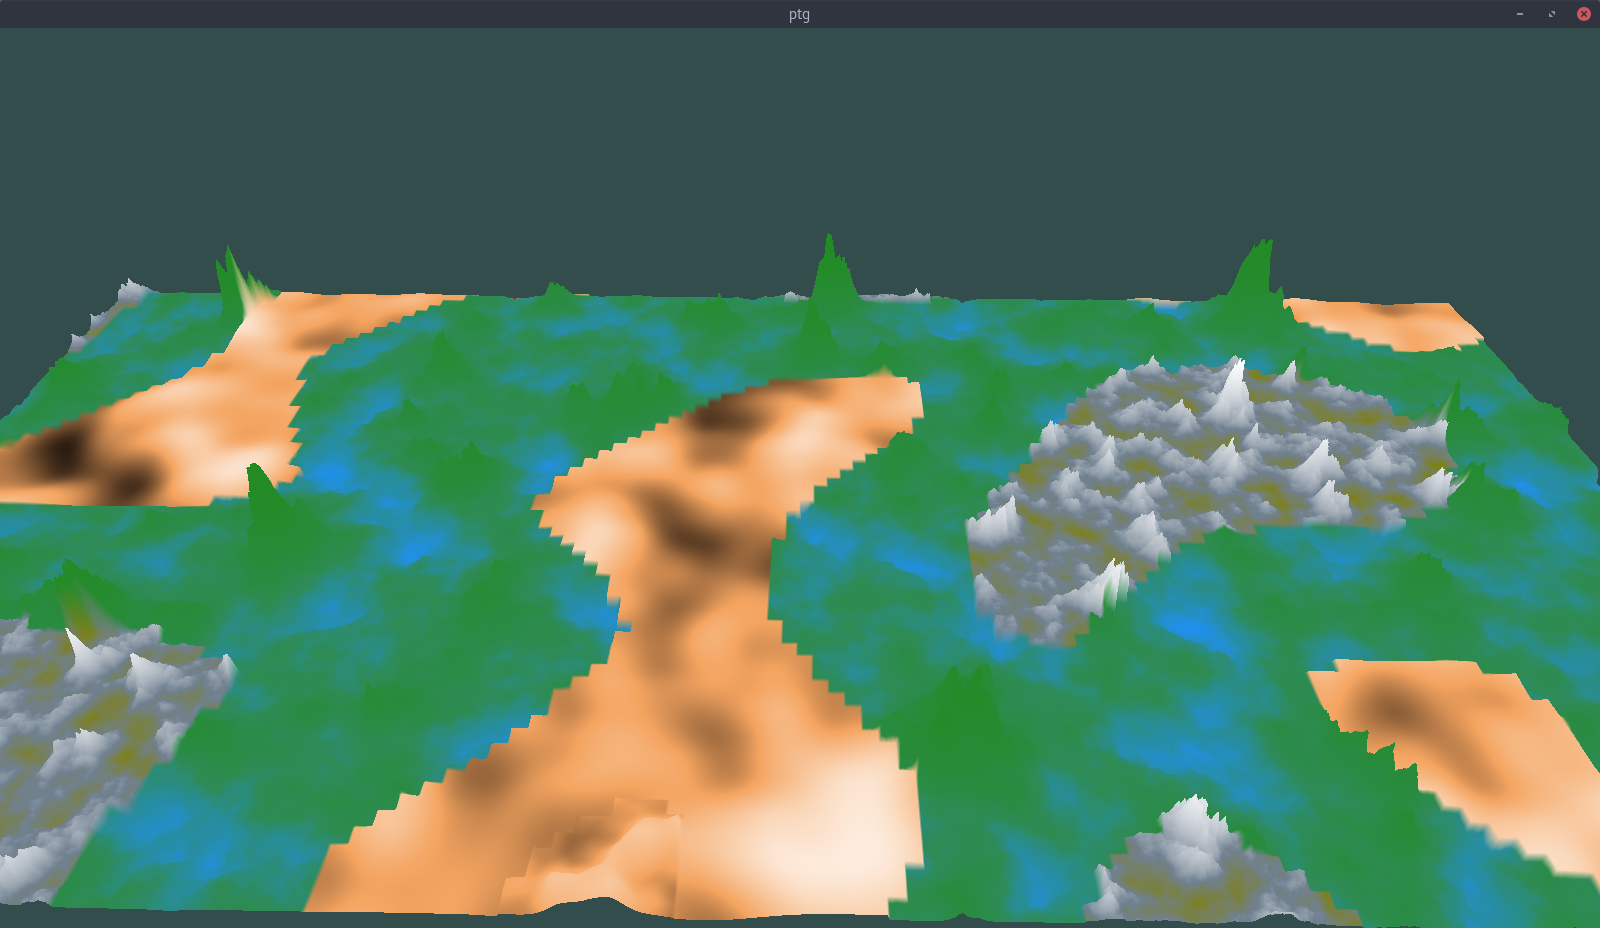
\includegraphics[width=.8\textwidth]{img/uffs/32b32.png}
        \caption{Frequência de Biomas = 32}
  \end{figure}
\end{frame}

\begin{frame}{Geração de Terrenos com Biomas Distintos para Jogos}
  \begin{figure}
		\centering
        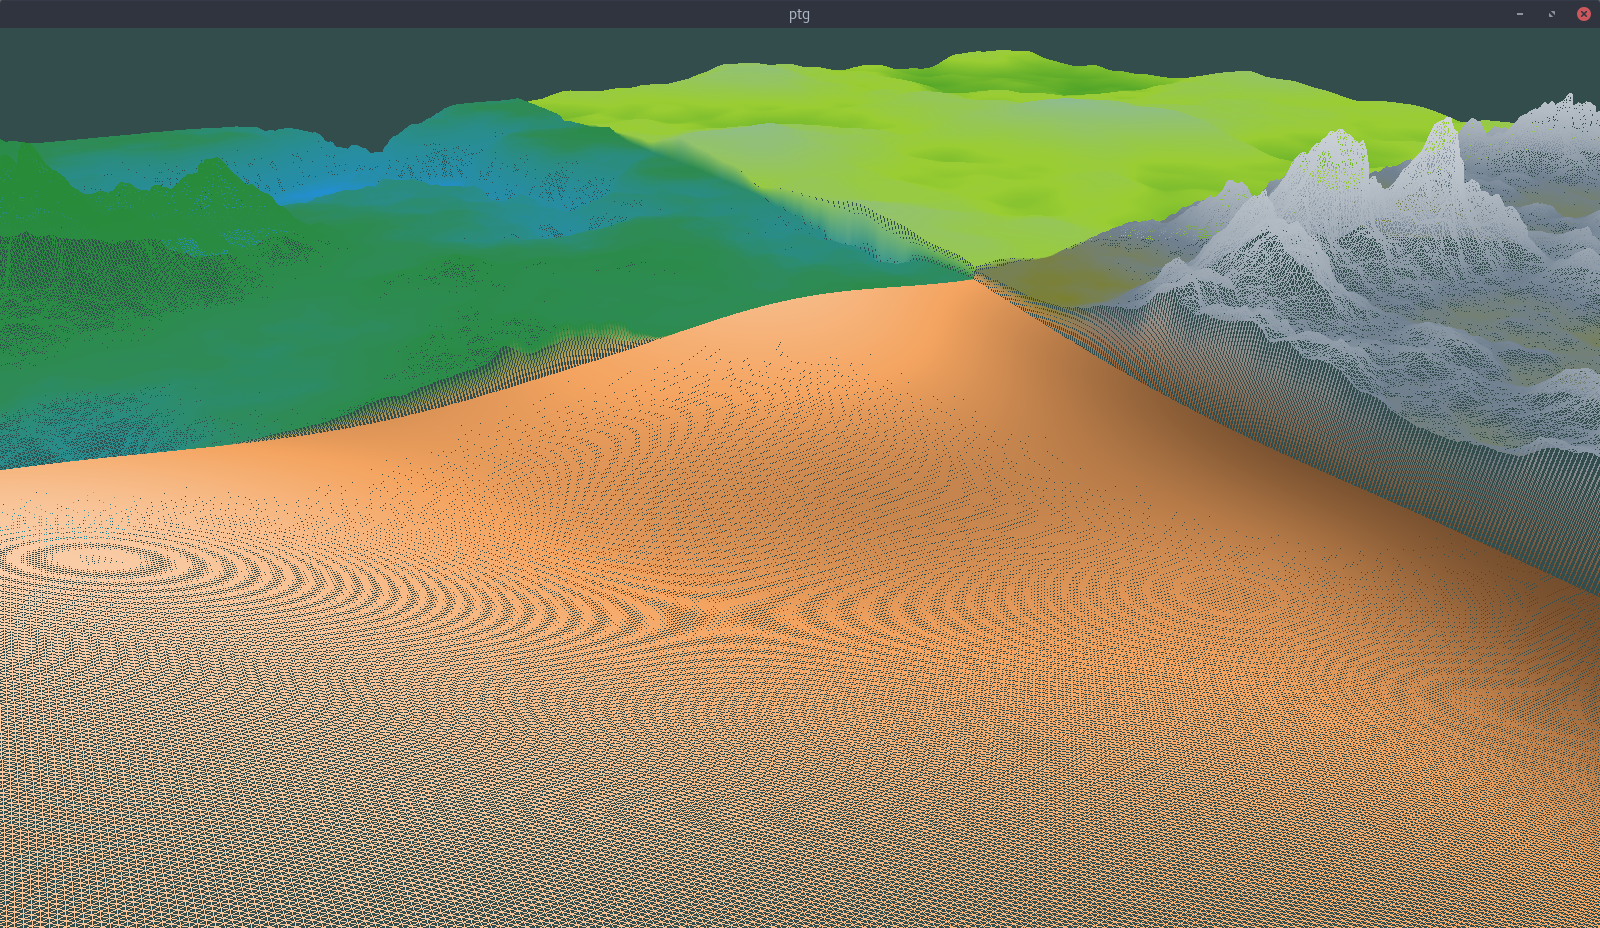
\includegraphics[width=.8\textwidth]
        {img/uffs/interpolationArea/notinter.png}
        \caption{Fronteiras descontínuas}
  \end{figure}
\end{frame}

\begin{frame}{Geração de Terrenos com Biomas Distintos para Jogos}
  \begin{figure}
		\centering
        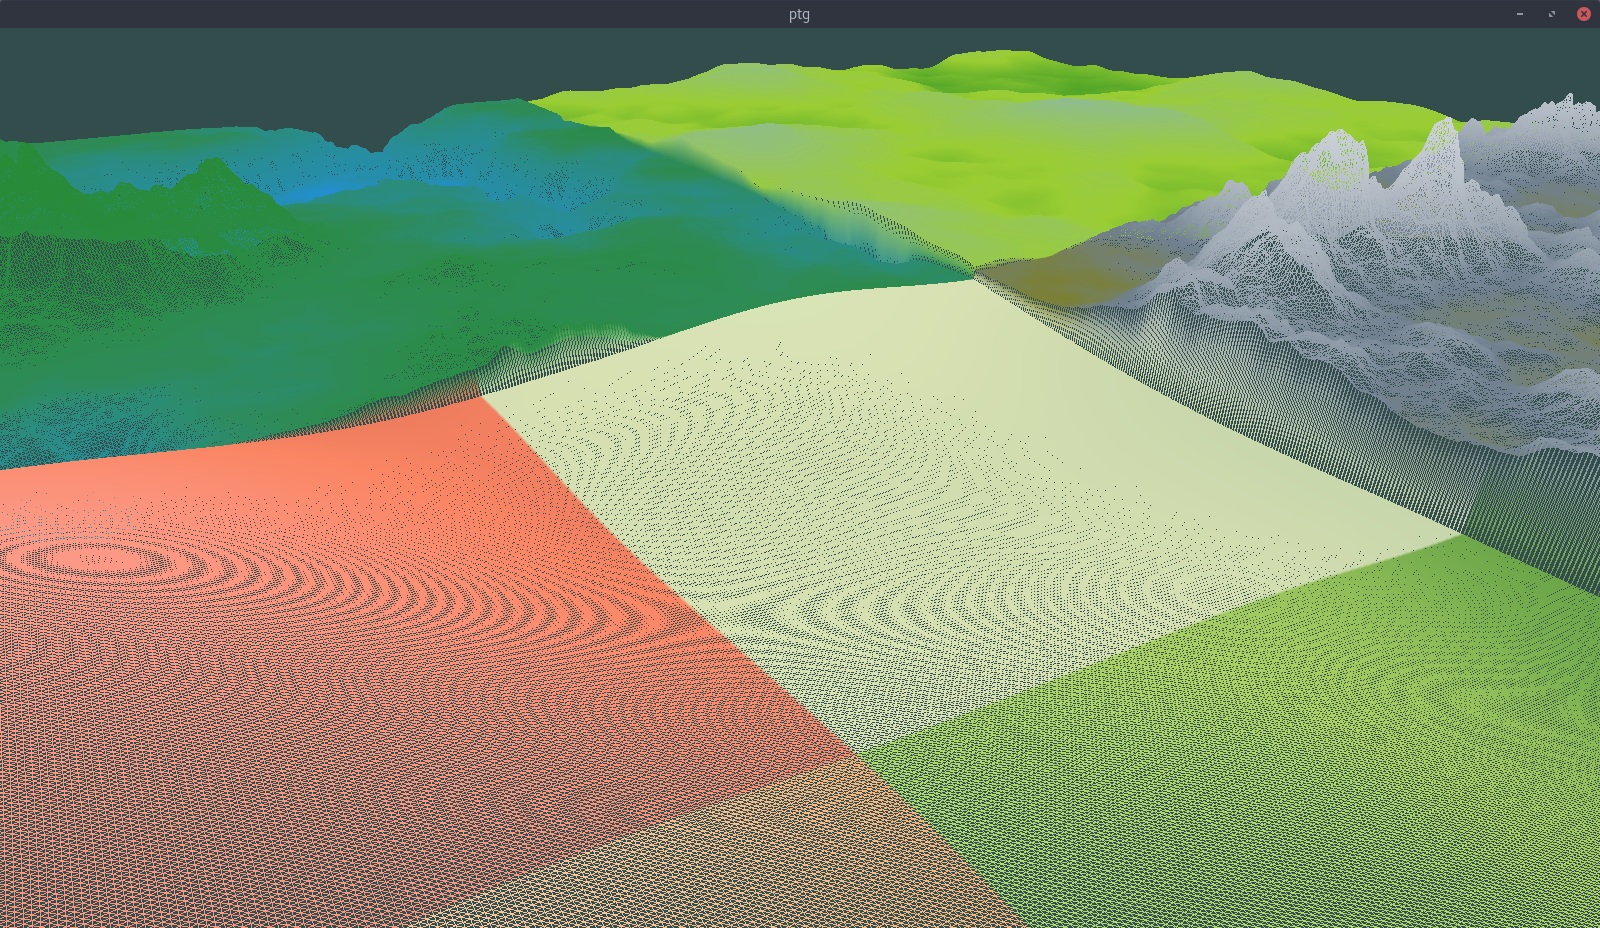
\includegraphics[width=.8\textwidth]
        {img/uffs/interpolationArea/showareanotinterpo.png}
        \caption{Casos de fronteiras}
  \end{figure}
\end{frame}

\begin{frame}{Geração de Terrenos com Biomas Distintos para Jogos}
  \begin{figure}
		\centering
        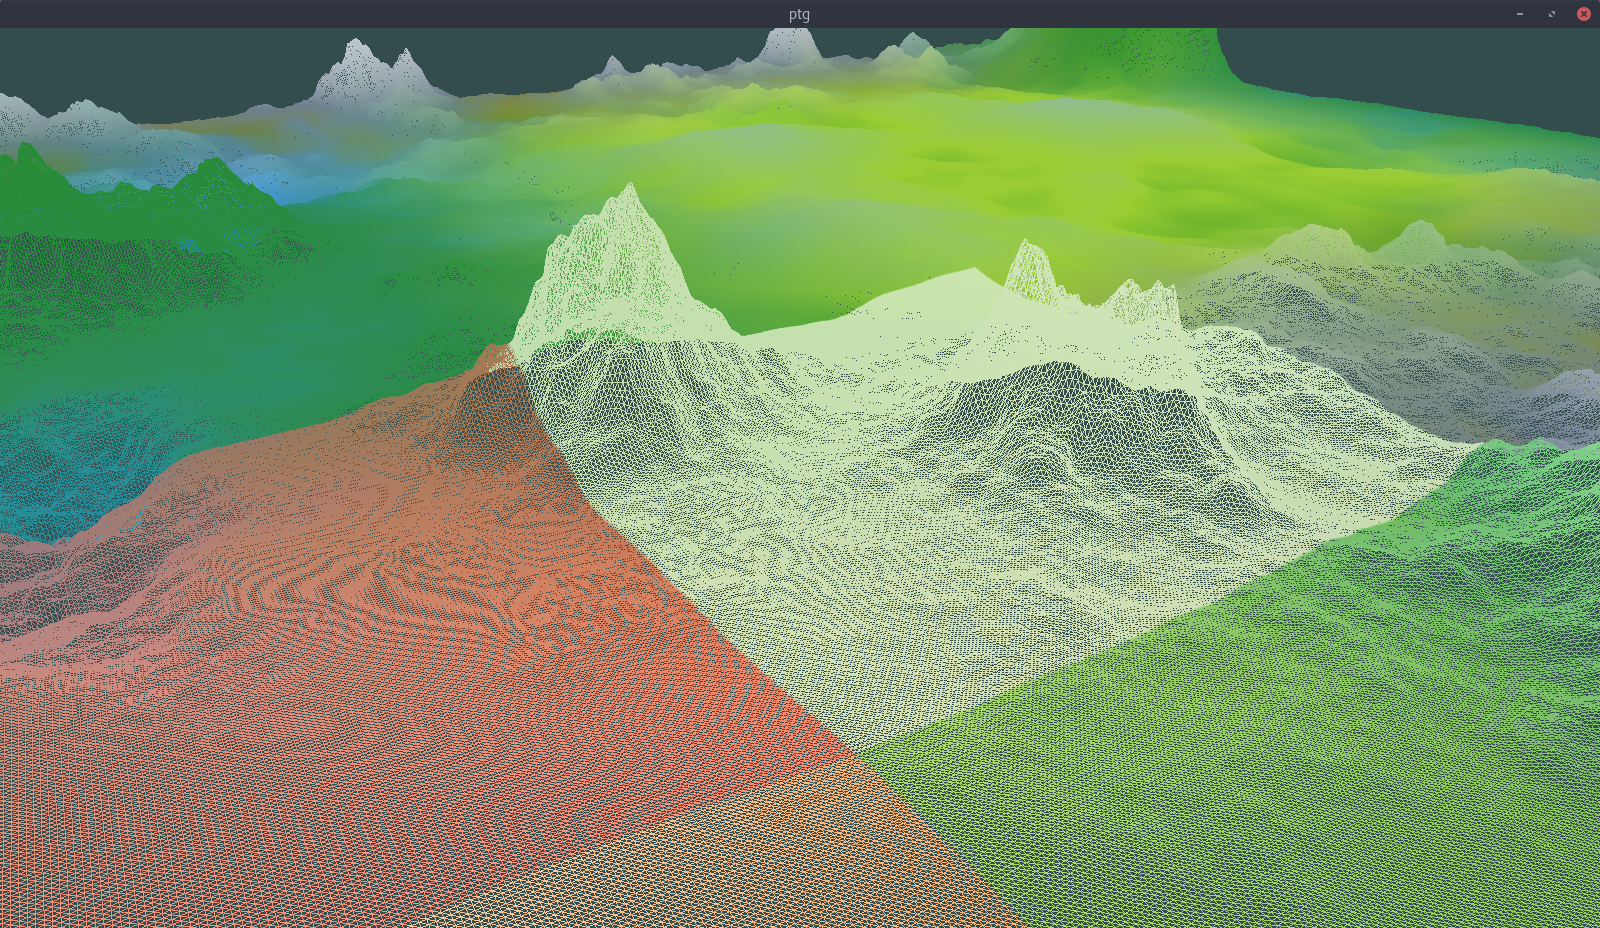
\includegraphics[width=.8\textwidth]
        {img/uffs/interpolationArea/showareainterpolating.png}
        \caption{Com interpolação}
  \end{figure}
\end{frame}

\begin{frame}{Geração de Terrenos com Biomas Distintos para Jogos}
    \begin{figure}
		\centering
        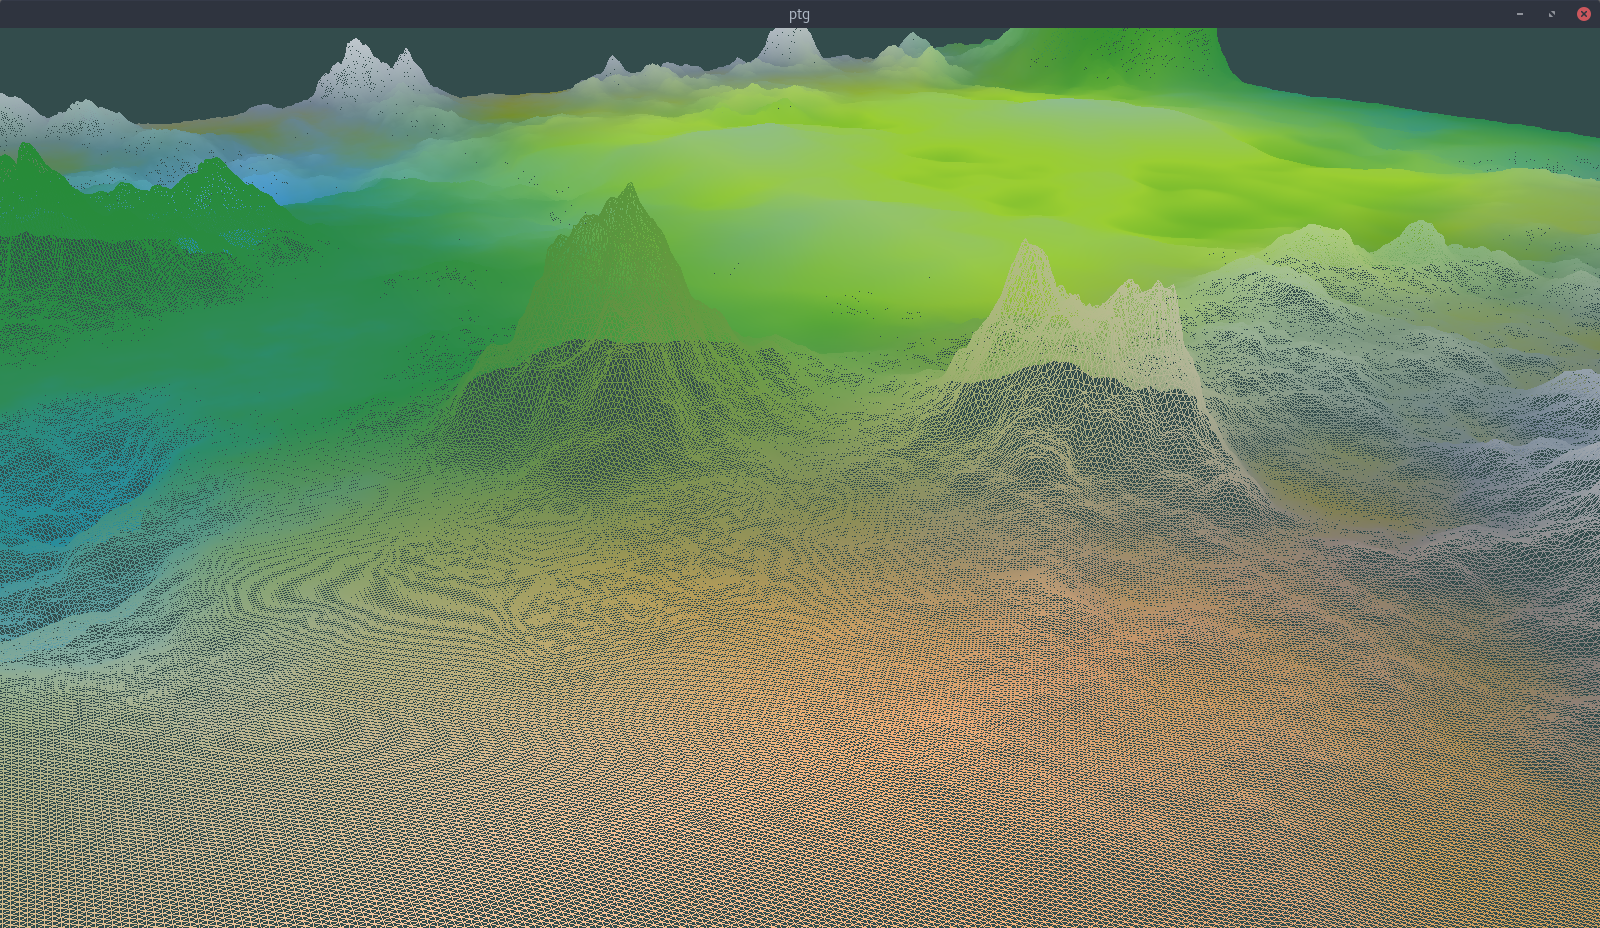
\includegraphics[width=.8\textwidth]{img/uffs/interpolationArea/interpolation.png}
        \caption{Com interpolação}
    \end{figure}
\end{frame}


% Trabalho do Fernando
\begin{frame}{Gerador de costas}
    \begin{figure}
		\centering
        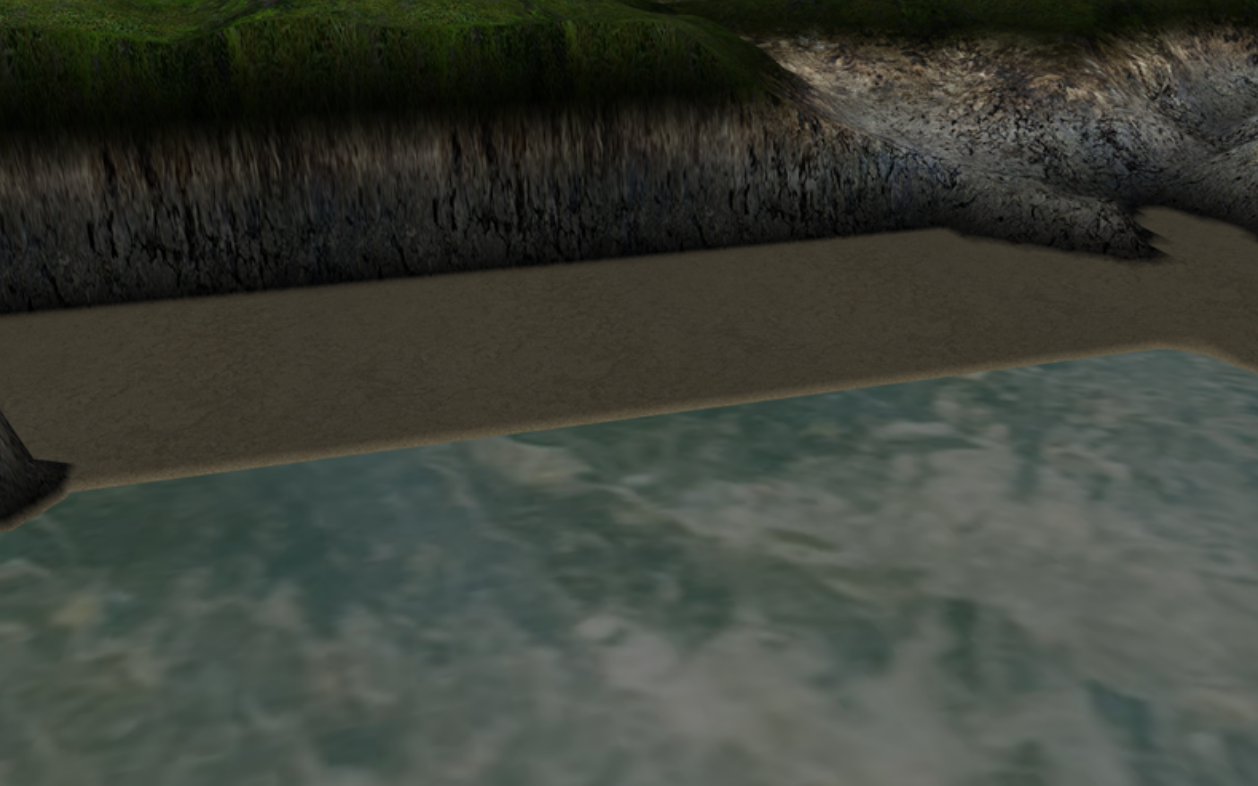
\includegraphics[width=.8\textwidth]{img/uffs/fernando/linearcosta.png}
        \caption{Costa linear.}
    \end{figure}
\end{frame}

\begin{frame}{Gerador de costas}
    \begin{figure}
		\centering
        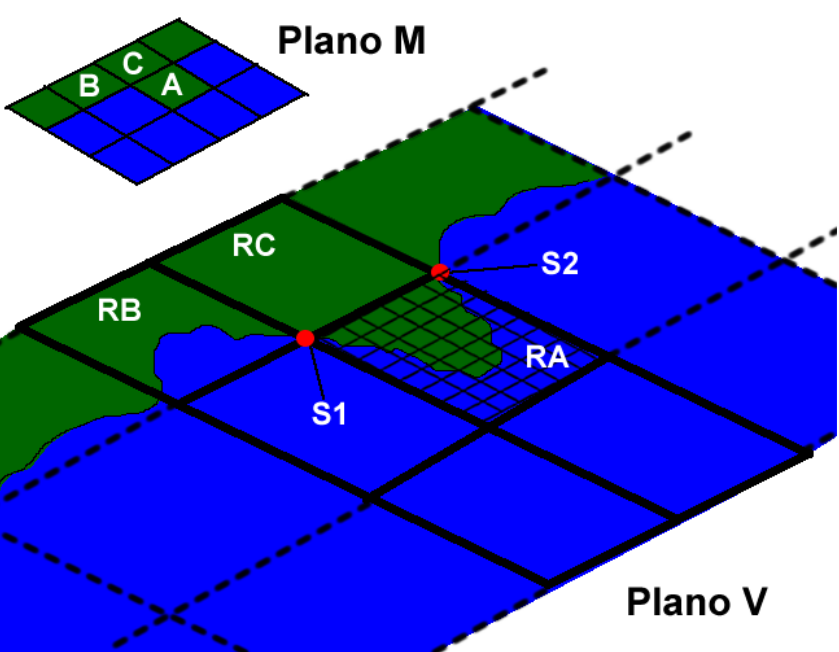
\includegraphics[width=.8\textwidth]{img/uffs/fernando/metodo.png}
        \caption{Método.}
    \end{figure}
\end{frame}

\begin{frame}{Fernando}
    \begin{figure}
		\centering
        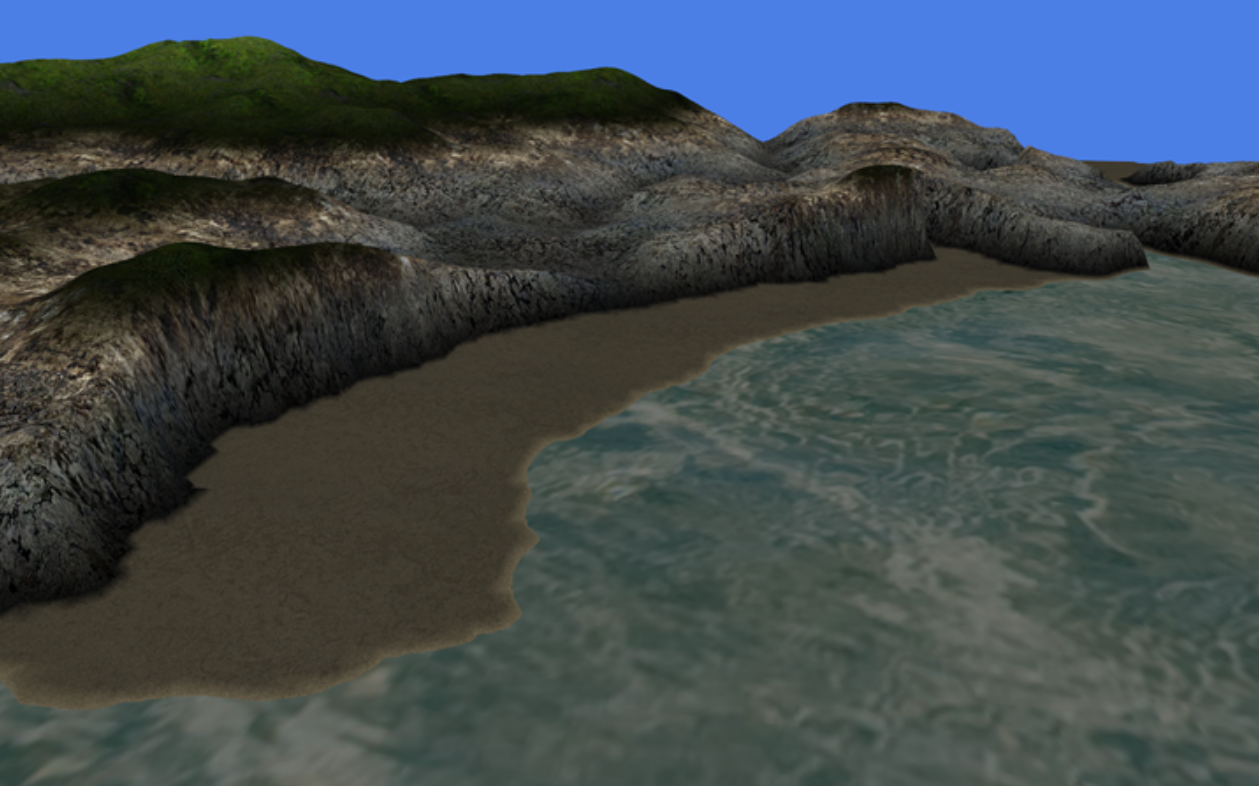
\includegraphics[width=.8\textwidth]
        {img/uffs/fernando/costaorganica.png}
        \caption{Costa orgânica.}
    \end{figure}
\end{frame}

\section{Jogos com Conteúdo Procedural}

\begin{frame}{Spore}
  \begin{itemize}
        \item Gera planetas esféricos com relevo procedural
        %To-do: por imagem do spore
    \end{itemize}
\end{frame}

% Usado para parar a contagem na barra de progresso e paginação
\appendix

{\setbeamercolor{palette primary}{fg=black, bg=white}
\begin{frame}[standout]
  Dúvidas?
\end{frame}
}

\begin{frame}[allowframebreaks]{Refêrencias}

  \bibliography{demo}
  \bibliographystyle{apalike}

\end{frame}

\end{document}
